\documentclass[hidelinks,msc,british]{ThesisPUC_uk}

\renewcommand{\subfigtopskip}{0in}
\renewcommand{\subfigcapskip}{0in}
\renewcommand{\subfigbottomskip}{0in}

%%%%%%%%%%%%%%%%%%%%%%%%%%%%%%%%%%%%%%%%%%%%%%%%%%%%%%%%%%%%%%%%%%%%%%%%%%%%%%%%

%\hyphenation{}

%%%%%%%%%%%%%%%%%%%%%%%%%%%%%%%%%%%%%%%%%%%%%%%%%%%%%%%%%%%%%%%%%%%%%%%%%%%%%%%%

%\usepackage[alf,abnt-etal-cite=2,abnt-etal-text=it]{abntex2cite}
\usepackage{url}
\usepackage{cite}
%\usepackage{natbib}
%\bibliographystyle{plainnat}

\usepackage{booktabs, multicol, multirow}
\usepackage{pdflscape}
\usepackage[section]{placeins}

\usepackage{rotating}
\usepackage{multirow}
\usepackage{amsmath}
\usepackage{mathrsfs}
\usepackage{array}
\usepackage{enumerate}
\usepackage{longtable}
\usepackage{pdflscape}
\usepackage[chapter]{algorithm}
\usepackage[skip=0pt]{caption}
\usepackage[noend]{algpseudocode}
\usepackage[justification=centering]{caption}
\usepackage[none]{hyphenat}

\usepackage{graphicx}
\usepackage{caption}
\usepackage{subfigure}
\usepackage{float}
 
\usepackage{commath}

%%%%%%%%%%%%%%%%%%%%%%%%
\usepackage{algorithmic,eqparbox,array}
\usepackage{algpseudocode}
\newcommand*\Let[2]{\State #1 $\gets$ #2}
\usepackage[noend]{algpseudocode}
\usepackage{xhfill}
\newcommand\Algphase[1]{%
\vspace*{-.7\baselineskip}\Statex\hspace*{\dimexpr-\algorithmicindent-2pt\relax}\xdotfill{0.4pt}%
\Statex\hspace*{-\algorithmicindent}\textbf{#1}%
\vspace*{-.7\baselineskip}\Statex\hspace*{\dimexpr-\algorithmicindent-2pt\relax}\rule{\textwidth}{0.4pt}%
}
\renewcommand\algorithmiccomment[1]{%
  \hfill\#\ \eqparbox{COMMENT}{#1}%
}
\newcommand\LONGCOMMENT[1]{%
  \hfill\#\ \begin{minipage}[t]{\eqboxwidth{COMMENT}}#1\strut\end{minipage}%
}

%%%%%%%%%%%%%%%%%%%%%%%%
\usepackage{xargs}                      % Use more than one optional parameter in a new commands
\usepackage[colorinlistoftodos,prependcaption,textsize=tiny]{todonotes}
\newcommandx{\fixme}[2][1=]{\todo[linecolor=red,backgroundcolor=red!25,bordercolor=red,#1]{#2}}
\newcommandx{\mynotes}[2][1=]{\todo[linecolor=blue,backgroundcolor=blue!25,bordercolor=blue,#1]{#2}}
%%%%%%%%%%%%%%%%%%%%%%%%

\newcommand{\q}[1]{``#1''}

\usepackage{comment}
\usepackage{fancyref}

% paragraph with a new line
\newcommand{\myparagraph}[1]{\paragraph{#1}\mbox{}\\}

\allowdisplaybreaks
\numberwithin{equation}{chapter}
\FloatBarrier

%%%%%%%%%%%%%%%%%%%%%%%%%%%%%%%%%%%%%%%%%%%%%%%%%%%%%%%%%%%%%%%%%%%%%%%%%%%%%%%%

\author{Nara Torres Moreira}
\authorR{Moreira, Nara T.}
\adviser{Marcus Vinicius Soledade Poggi de Arag\~ao}
\adviserR{Poggi, Marcus}
\title{Timetabling}
\titulo{Actual Solutions for School Timetabling Problem Through Integer Programming}
\day{10th} \month{March} \year{2015}

\city{Rio de Janeiro}
\CDD{004}
\department{Informatics}
\program{Graduate}
\school{Department of Informatics}
\university{Pontif\'{i}cia Universidade Cat\'{o}lica do Rio de Janeiro}
\uni{PUC-Rio}
%\degree{Master in Informatics}

%%%%%%%%%%%%%%%%%%%%%%%%%%%%%%%%%%%%%%%%%%%%%%%%%%%%%%%%%%%%%%%%%%%%%%%%%%%%%%%%

\jury{%
  \jurymember{}{Departamento de Inform\'atica -- PUC-Rio}%
	%\schoolhead{}%
}

%%%%%%%%%%%%%%%%%%%%%%%%%%%%%%%%%%%%%%%%%%%%%%%%%%%%%%%%%%%%%%%%%%%%%%%%%%%%%%%%

\resume{
}

%%%%%%%%%%%%%%%%%%%%%%%%%%%%%%%%%%%%%%%%%%%%%%%%%%%%%%%%%%%%%%%%%%%%%%%%%%%%%%%%



%%%%%%%%%%%%%%%%%%%%%%%%%%%%%%%%%%%%%%%%%%%%%%%%%%%%%%%%%%%%%%%%%%%%%%%%%%%%%%%%

\acknowledgment{%

}

%%%%%%%%%%%%%%%%%%%%%%%%%%%%%%%%%%%%%%%%%%%%%%%%%%%%%%%%%%%%%%%%%%%%%%%%%%%%%%%%

\abstract{%

}

\keywords{
  \key{Timetabling}%
}

%%%%%%%%%%%%%%%%%%%%%%%%%%%%%%%%%%%%%%%%%%%%%%%%%%%%%%%%%%%%%%%%%%%%%%%%%%%%%%%%

\resumo{%

}

\chaves{
	\chave{Actual Solutions for School Timetabling Problem Through Integer Programming}%
}

%%%%%%%%%%%%%%%%%%%%%%%%%%%%%%%%%%%%%%%%%%%%%%%%%%%%%%%%%%%%%%%%%%%%%%%%%%%%%%%%

\tablesmode{figtab} % none, fig, tab ou figtab

%%%%%%%%%%%%%%%%%%%%%%%%%%%%%%%%%%%%%%%%%%%%%%%%%%%%%%%%%%%%%%%%%%%%%%%%%%%%%%%%

\dedication{}

%%%%%%%%%%%%%%%%%%%%%%%%%%%%%%%%%%%%%%%%%%%%%%%%%%%%%%%%%%%%%%%%%%%%%%%%%%%%%%%%

%\epigraph{}
%\epigraphauthor{}
%\epigraphbook{}

%%%%%%%%%%%%%%%%%%%%%%%%%%%%%%%%%%%%%%%%%%%%%%%%%%%%%%%%%%%%%%%%%%%%%%%%%%%%%%%%

\begin{document}

\chapter{Introduction}
\label{chap:intro}

%%%%%%%%%%%%%%%%%%%%%%%%%%%%%%%%%%%%%%%%%%%%%%%%%%%%%%%%%%%%%%%%%%%%%%%%%%%%%%%%%%

Here the ideas discussed in this dissertation are contextualized. Giving this, a brief introduction, some definitions and main variants to the Timetabling Problem (TTP) are provided.

% ------------------------------------------------------------
\section{Introducing the basic timetabling problem}

\mynotes{DSS, Bilkent, Guenalay and Sahin, Guenalay2006, \cite{Guenalay2006}}
Timetabling problems are an example of the types of practical scheduling problems faced by many organizations, including universities. The problem can be described as needing to schedule a given number of lectures, involving both teachers and classrooms, over a fixed period of time (typically a week), while sometimes having to satisfy a set of additional constraints of various types. The problem is known to be a hard problem and therefore many researchers have shown an interest in it since the early 1960's. Schaerf \cite{Schaerf99} showed that the problem is NP-complete and that exact optimal solution could be obtained only for small size problems.

Although the original problem was set in the school environment, it now finds a wide range of application to areas from sport event timetabling to transportation timetabling studies.


% ------------------------------------------------------------
\section{Brazilian school timetabling problem}



% ------------------------------------------------------------
\section{Practical and realistic formulation}

\mynotes{Purdue University, \cite{Murray2007}}
It is a widely studied area and many potentially useful algorithms have been offered for solving the university course timetabling problem. Unfortunately, much of the work in this area has been conducted using artificial data sets or based on actual problems that have been greatly simplified. Methods developed have also rarely been extended to the solution of actual university problems of any large scale, instead most were restricted to a single department or school.

The major differences between many of the problems studied and their real life counterparts are the additional complexity imposed by course structures, the variety of constraints imposed, and the distributed responsibility for information needed to solve such problems at a university-wide level.

As pointed out in \cite{Murray2007}, the biggest obstacle to solving actual university course timetabling problems is that the complexity can increase considerably beyond that represented in standard formulations of the problem. As the complexity increases, it is easy to be caught in the dual bind that the problem is both more challenging to develop an effective solution approach for, and this approach is less likely to be usable on other university timetabling problems.

As observed by Carter \cite{Carter2001}, there are few published papers that described actual implementations of course timetabling. From what we know, the first example of an automated and integrated course timetabling and student scheduling system across a institution was developed for the University of Waterloo between 1979 and 1985. Although the system was implemented 29 years ago, much of the discussion is still very relevant. By 2001, Carter expressed at \cite{Carter2001} his belief that there was still no system for solving the large-scale course timetabling problem with such level of mathematical sophistication.

By 2006, Guenalay and Sahin introduced at \cite{Guenalay2006} a Decision Support System (DSS) for the university timetabling that allows the direct involvement of the decision maker. They affirmed that their model was the first one which simultaneously combined such a DSS approach with a goal programming optimization tool.

\fixme{citar software!}


% ------------------------------------------------------------
\section{Main similar formulations and their differences}

For solving the high school timetabling problem, this work is based on an integer programming formulation together with strategies for helping at the convergence in the best solution search process.

Among the existing published works that considered more realistic formulations for high school timetabling problems, we highlight \cite{Birbas2009} and \cite{Birbas2009} as those whose embraced problems were the most similar to the one considered in this work. Several practical issues emphasized by them were also identified during TRIEDA's development and were referenced along this work.

Still, there are differences between their timetabling problems and the one here presented. Following, the major points are listed.
-
-
-

Further differences can be identified along this work.

Because TRIEDA is a commercial software, it has been developed to be as portable and flexible as possible. Particularly, the system embraces most common rules and cases found in Brazilian universities and schools.


% ------------------------------------------------------------
\section{Data accuracy and Politics}

\mynotes{from \cite{Murray2007}}
Timetabling is a resource allocation problem; therefore, at most universities responsibility for constructing the timetable is distributed among the academic units with the faculty, physical facilities, and other resources required for offering instruction. Murray, M\"{u}ller and Rudov\'{a} observe at \cite{Murray2007} that providing support for this distributed responsibility is important because departmental timetablers have a much more intimate knowledge of the needs of the courses offered, the professor who might be able to teach a particular class, and the spaces available for specialized instruction than any database that might be maintained centrally. Maintaining each department's sense of ownership in the timetables that are produced is also an important factor in their acceptance of the solutions produced by an automated timetabling process. They say the process needs to be one that assists them rather than replaces them.

Obtaining coherent and correct data is a particular important and sensitive issue. Because data accuracy depends on each department, it is extremely important that data collection phase of an automating process has a deep involvement of all of those who usually operate in the traditional manual process. Any inaccuracy of data can result in a bad or even non-deployable solution.

\fixme{citar funcionalidade: motivos de nao atendimento}

Murray, M\"{u}ller and Rudov\'{a} tells at \cite{Murray2007} that inequity in the quality of time and room assignments received by different departments and faculty members doomed a previous attempt at automating the timetabling process at Purdue University. A similar situation was faced by TRIEDA in July of 2014 while an attempt of deploying a solution in a Brazilian university.

Automating people assignments is different from automating other process --- the optimization factor is definitely \textbf{not} more important than people satisfaction. Only keeping that in mind it is possible to obtain an actual deployable solution.

As wisely pointed out in \cite{Carter2001}, practical course timetabling is 10\% graph theory, and 90\% politics. Carter tells that when they first began designing the system for University of Waterloo, they were warned: \q{You can not dictate to professors when they will teach courses}. Consequently, they were told that course timetabling could not work. Or, more precisely, they can not assume that the timetable can use a clear slate. There are many possible reasons for this. Part-time professors may be available only on certain days or times. University professors often have other commitments and industrial research projects. Teaching is only a part of their job, and probably less than half of their time is devoted to teaching.

It follows that it is essential to allow professors to restrict their available timetables as much (or as little) as they want.

Guenalay and Sahin described at \cite{Guenalay2006} an approach for university timetabling with a goal programming optimization tool in order to process the instructor teaching time preferences. As they observed, using a multi-objective decision making model to solve the problem, and hence considering instructor preferences by using weights, cannot be considered consistently reliable. Such approach unifies the disparate goals of the model, but depends on very subjective choice of weights.

Professors' availabilities and preferences issue should therefore not be underestimated.


The primary design goal is to assist academic timetablers with the problem of building a good timetable, not necessarily finding a true optimal solution.


% ------------------------------------------------------------
\section{Timetabling Conferences}




% ------------------------------------------------------------

This is a test reference to \cite{Carter2001}.    % Waterloo, Canada
This is a test reference to \cite{Murray2007}.    % Purdue (unitime), USA
This is a test reference to \cite{Unitime}.       % website
This is a test reference to \cite{DSS}.           % website
This is a test reference to \cite{Guenalay2006}.  % Bilkent, Turkey, (DSS)
This is a test reference to \cite{Schaerf99}.  		% Schaerf99
This is a test reference to \cite{Michael2002}.   % Michael2002
This is a test reference to \cite{SchoolOverview2010}.   % SchoolOverview2010
This is a test reference to \cite{Birbas2009}.    % Birbas2009
This is a test reference to \cite{Mimosasoftware}.
This is a test reference to \cite{Patat}.
This is a test reference to \cite{Hstt}.				  % Benchmarking project for highschool
This is a test reference to \cite{ITC2007}.				% International Timetabling Competition
This is a test reference to \cite{Ectt}.					% Udine, Italy
This is a test reference to \cite{Udine}.
This is a test reference to \cite{Watt}.					% Working group on automated timetabling




%%%%%%%%%%%%%%%%%%%%%%%%%%%%%%%%%%%%%%%%%%%%%%%%%%%%%%%%%%%%%%%%%%%%%%%%%%%%%%%%%%

\section{Dissertation Outline}
This work is organized as follows: 
\begin{itemize}
	\item Chapter \ref{chap:timetabling} introduces Trieda's timetabling problem.
	\item Chapter \ref{chap:mipformulation} shows the mathematical formulation for the problem.
	\item Chapter \ref{chap:strategies} presents different approaches and strategies for solving the MIP formulation.
	\item Chapter \ref{chap:constranalysis} analyzes the impact of some requirements in the MIP solving.
	\item Chapter \ref{chap:converting} presents an attempt to converting a XHSTT format into a Trieda's problem format.
	\item Chapter \ref{chap:conclusions} contains the conclusions of this work.
\end{itemize}
\chapter{Trieda's Timetabling Problem}
\label{chap:timetabling}


School timetabling problems vary a lot from country to country. This chapter provides a complete definition to the timetabling problem for Brazilian elementary education system considered in this dissertation.


%%%%%%%%%%%%%%%%%%%%%%%%%%%%%%%%%%%%%%%%%%%%%%%%%%%%%%%%%%%%%%%%%%%%%%%%%%%%%%%%%%

\section{Introducing the system}
\label{sec:system}


TRIEDA is an academic planning system for educational institutions, designed as a multi-user application with a completely web-based interface. Unlike many academic planning systems and timetabling researches, which consider simplifications of the actual problem, TRIEDA makes all necessary decisions so that a complete, optimized and applicable solution is provided.

Timetabling problems vary a lot depending on the kind of educational institution. The system has nowadays two distinct modules: one for solving high school timetabling problems and another for solving university timetabling problems. For each one, TRIEDA uses a completely different solver. This dissertation focus only on the high school module.

The system is based on a \q{demand-drive} philosophy where students first chose their courses, and having knowledge of the complete institution structure and available resources, the aim is to provide a complete and feasible solution that maximizes the number of satisfied requests while respecting a set of didactic-pedagogical requirements. For the university module, reducing costs is also strongly aimed. For the school module, some didactic-pedagogical requirements together with professors satisfaction are usually the most important issues.


\subsection{Simulation usability}
\label{subsec:simulation}

Carter tells us in \cite{Carter2001} that, in the Fall of 1988, the University of Waterloo opened the Davis Building. A total of 40 (smaller) classrooms across campus were replaced by 30 generally larger classrooms in the new building. The number of rooms decreased, but the total number of seats increased. The Scheduling Office was very concerned about how the new space would impact space allocation. A timetabling automated system developed for the university effectively was used for simulating the new scenario and solved a potentially serious planning problem.

Therefore, as was exemplified, the timetabling system can also be used as a fast \q{What if?} tool to evaluate proposed changes in resources or institution rules.


\subsection{Multiple scenarios}
\label{subsec:scenarios}

Through the system interface the user can easily register each entity and resource of the institution and its quality requests. The set of all registered information for the problem defines a scenario. The system allows each user to create and manage multiple scenarios, which is very useful when comparing and evaluating the impact of different situations.

Registering data through the interface can be done manually one by one or importing Excel spreadsheets. Similarly, solution is graphically available for analysis through the interface or can also be exported to Excel spreadsheets.


\subsection{Interface and solver interaction}
\label{subsec:interaction}

Interaction between the user interface and the solver is made by XML files. Once all problem data is registered by the user such that one has a consistent scenario, an optimization request can be made. Such request generates a XML input file and calls the solver, which reads the input file, loads data and starts the optimization process. Once the final solution is obtained, a XML output file is written and the solver process is ended. Following, the application loads the solution and user interface shows all results.


\subsection{Manual changes}
\label{subsec:manual}

A very common requirement in logistic and planning systems is to allow the user to make manual changes in a solution. TRIEDA allows user to manually create new classes or modify existing classes, as long the result does not violate basic and necessary operational constraints.


\subsection{Non--satisfaction reasons}
\label{subsec:reasons}

As discussed in section ~\ref{sec:accuracy}, data quality is essential for obtaining a good, feasible and applicable solution. Unfortunately, data inaccuracy is though very frequent and therefore the system should be prepared to deal with it, as long it is possible.

Besides the possibility of data inaccuracy, it can be hard to affirm if the demand of a scenario can be fully satisfied, specially when it is a large instance. Analyzing both input data and solution for a real world problem is a hard task. As an user auxiliary functionality for solution analysis, the system exhibits for each non--satisfied demand possible explanations for the non-allocation, which can help both to identify input data errors and to understand resources limitations.


\subsection{Virtual professor tips}
\label{subsec:tips}

Because there is in general no insurance that there are enough teaching resources for fully satisfying the demand, the concept of virtual teaching resource is used (see ~\ref{defpv}). Virtual resources should though be used as little as possible.

An extra functionality of the system for helping the user while managing a solution is called \q{virtual professors tips}. For each virtual professor assigned to a solution class, it may be exhibited a tip or a suggestion for a change in some professor availability that would lead to a possible substitution of that virtual resource for a real professor. This can be quite useful for scenarios where professors availability is very limited, but it is ineffective when professors are full-time.



%%%%%%%%%%%%%%%%%%%%%%%%%%%%%%%%%%%%%%%%%%%%%%%%%%%%%%%%%%%%%%%%%%%%%%%%%%%%%%%%%%

\section{Introducing the school timetabling problem}
\label{deftriedaschool}

% explain trieda's general problem and what must be assigned

Unlike university problems, high school's students have low or no freedom at all in their choices for courses. Usually students are previously clustered into sections, in the sense that if two students are in the same section, then they have the same demands and should attend to the same lessons. Therefore, in a school timetabling problem the number of sections per course is known and assignments are made for each pre--defined cluster of students instead of for each single student.

Besides, in high school, sections usually have pre--assigned rooms. This is not an obligation though. For practical courses, it is common that several sections attend to lessons at the same laboratory. For sport classes, it is even common that two or more classes simultaneously share a physical space, like a sports court. But indeed, only in a minority of cases shared rooms are involved.

A solution is composed of a set of courses sections that should be offered in order that demands are satisfied. For each course section it must be decided:

\begin{itemize}
\item the classroom where section's lessons take place. Usually each section has a single possible room, but for practical courses it is to be decided;
\item the time slots of each lesson;
\item the professor assigned to the section;
\end{itemize}

No incomplete solution is acceptable.

The planning horizon, or \textit{teaching period}, is a week. It refers to the timetable duration, so that it is considered that classes don't change from a week to another in the same year or planning term.
 


%%%%%%%%%%%%%%%%%%%%%%%%%%%%%%%%%%%%%%%%%%%%%%%%%%%%%%%%%%%%%%%%%%%%%%%%%%%%%%%%%%

\section{Entities and Concepts}
\label{sec:entities}


%%%%%%%%%%%
% Horario-Dia
\paragraph{Time slot}
\label{deftimeslot}

Each time slot has a beginning time, an ending time and a weekday. For instance, Monday from 14:00 to 14:50. Besides, time slot duration is the number of minutes between the beginning and ending time of a time slot.


%%%%%%%%%%%
% Semana Letiva
\paragraph{Calender Timetable}
\label{deftimetable}

Corresponds to the way a school term week is split in the sense of shifts (see ~\ref{defshift}) and time slots.

Table ~\ref{tab:calendarioMT} shows an example of timetable with $2$ shifts (morning and afternoon), each one with $4$ class-times and a 30-minutes break between the $2$ first class-times and the $2$ last class-times of the shift. All class-times have $50$ minutes duration. From Monday to Friday all time slots are available, on Saturday only the morning time slots are available and on Sunday no time slot is available (unavailability is represented by a dash).

\begin{table}[H]
\centering
\begin{tabular}{l|c|r|r|r|r|r|r|r}
Shifts & Time Slots & Mon & Tue & Wed & Thu & Fri & Sat & Sun \\\hline
MORNING & 08:00 to 08:50 & & & & & & & - \\
MORNING & 08:50 to 09:40 & & & & & & & - \\
MORNING & 10:10 to 11:00 & & & & & & & - \\
MORNING & 11:00 to 11:50 & & & & & & & - \\
AFTERNOON & 14:00 to 14:50 & & & & & & - & - \\
AFTERNOON & 14:50 to 15:40 & & & & & & - & - \\
AFTERNOON & 16:10 to 17:00 & & & & & & - & - \\
AFTERNOON & 17:00 to 17:50 & & & & & & - & -
\end{tabular}
\caption{\label{tab:calendarioMT}Morning-Afternoon Timetable.}
\end{table}

It is possible to register as many timetables as necessary. This way, besides the timetable at ~\ref{tab:calendarioMT} we can \textit{also} have the one at ~\ref{tab:calendarioTN}. 

This timetable also has time slots in $2$ shifts, now afternoon and evening, but here class-times have $60$ minutes duration. It has $3$ class-times in the Afternoon shift and $4$ class-times in the Evening shift, the break-times are completely different from break-times of Morning-Afternoon Timetable, and there is not time slot available at weekends (Saturday and Sunday).


\begin{table}[H]
\centering
\begin{tabular}{l|c|r|r|r|r|r|r|r}
Shifts & Time Slots & Mon & Tue & Wed & Thu & Fri & Sat & Sun \\\hline
AFTERNOON & 13:00 to 14:00 & & & & & & - & - \\
AFTERNOON & 14:00 to 15:00 & & & & & & - & - \\
AFTERNOON & 15:00 to 16:00 & & & & & & - & - \\
EVENING & 18:00 to 19:00 & & & & & & - & - \\
EVENING & 19:00 to 20:00 & & & & & & - & - \\
EVENING & 20:20 to 21:20 & & & & & & - & - \\
EVENING & 21:20 to 22:20 & & & & & & - & -
\end{tabular}
\caption{\label{tab:calendarioTN}Afternoon-Evening Timetable.}
\end{table}


Time slots of the same timetable must have the same duration and can not overlap each other. Time slots of different timetables are independent: they can be completely different and even overlap, as the examples have shown.


%%%%%%%%%%%
\paragraph{Shift}
\label{defshift}

A shift is a label for a set of slot times.

It is mandatory that every time slot of a timetable belongs to some shift; a timetable can have time slots of different shifts; and a shift can have time slots of distinct timetables.

There is no constraint for associating a time slot and a shift, which means that a shift can be seen simply as a label (usually called ``Morning'', ``Afternoon'', ``Evening'', ``Integral'', ``Morning-Afternoon'', etc) and time slots of the same shift can overlap each other or have distinct durations.

The main role of the concept of shift is to define at which time slots a student can have classes, as discussed in section ~\ref{constrstudentsched}.


%%%%%%%%%%%
% Session of a day
\paragraph{Session of a day}
\label{defsession}

Sessions of the day are the commonly known concept for Morning, Afternoon or Night. The concept of sessions of day is necessary only to assist in obtaining compact timetables for professors. 


%%%%%%%%%%%
\paragraph{Course}
\label{defcourse}

A \textit{course} is a ``chair'' or ``subject'' that a student can take.
paragraph
Common examples in high-school are ``Mathematics'', ``Geography'' or ``Biology''.

Every course has a total number of credits per week, with all the credits necessarily having the same duration. This means that if the student John Mayer takes classes of a course with $N$ credits of $50$ minutes duration, exactly $N$ time slots of $50$ minutes of John's week schedule must be assigned to lessons of this course.

Every course has a set of time slots to which it can be assigned. These time slots can belong to different timetables, as long they have the same duration.

Every course can be assigned to a specific set of classrooms where it can be held. If there is no specific classroom associations, it is assumed that the course can be held in any classroom.


%%%%%%%%%%%
\paragraph{Curriculum}
\label{defcurric}

A \textit{curriculum} is the set of all courses token by a student at a specific school studying year.


%%%%%%%%%%%
\paragraph{Campus, Block and Classroom}
\label{defclassroom}

The basic physical structure of a university is formed by:
\begin{itemize}
\item \textit{Classroom}: room where classes can be held.
\item \textit{Block}: set of classrooms, usually of the same building.
\item \textit{Campus}: each campus has a set of blocks, besides other features.
\end{itemize}


%%%%%%%%%%%
\paragraph{Offer}
\label{defoffer}
 
An \textit{offer} is made of a curriculum, shift and campus. Its interpretation is that courses of this curriculum are offered at the campus at the specific shift.


%%%%%%%%%%%
\paragraph{Demand}
 \label{defdem}

A \textit{demand} is made of a set of students, an offer and a course. Its interpretation is that this set of students, associated with the specified offer, should attend to the specified course.
For instance, a set of $40$ students associated with the ``COMP-AFT'' offer demands for the course ``Calculus I''.


%%%%%%%%%%%
\paragraph{Student--Demand}
\label{defstdem}

A student--demand is an individual request of a student for a course. It is made of a student and a demand.


%%%%%%%%%%%
\paragraph{Class}
\label{defclass}

A class refers to the same group of students that will be taught a set of courses.


%%%%%%%%%%%
\paragraph{Lesson}
\label{deflesson}

A lesson refers to a particular course being taught to a class by a teacher at some period of a day.


%%%%%%%%%%%
\paragraph{Section}
\label{defsection}

A \textit{section of a course} is a class (set of students) and its associated set of lessons for the course.

In a complete and feasible solution, each course section has the following attributes:
\begin{itemize}
\item a set of students (class);
\item a classroom where the lessons take place;
\item time slots for each course lesson, totaling the number of credits of the course;
\item a professor who teaches the lessons.
\end{itemize}


%%%%%%%%%%%
\paragraph{Professors}
\label{defprof}

Each professor is a teaching staff resource that can be assigned to classes, according to its features. Every professor has:
\begin{itemize}
\item its own available timetable,
\item a list of courses that he/she is capable of teaching,
\item a priority number, 1 or 2, that indicates how important is that professor for the institution.
\end{itemize}




%%%%%%%%%%%
\paragraph{Virtual Professors}
\label{defpv}

The most basic solution restrictions are based on resources availabilities. There is no assurance in general there are enough professors to meet the hole demand. Therefore, the concept of \textit{virtual professor} is introduced.

Each \textit{virtual professor} means the hiring of a new professor by the institution. Whenever there is no feasible solution with full satisfied demand due to absence of professors, and only in this situation, virtual professors should be created by the solver and used until demand is fulfilled.

Since a virtual professor is just a prediction of a new profile, it has default settings, full-available timetable and is not considered at some professor quality restrictions.

The need of virtual teaching resources is also due to the usual floating feature of professors availability.


%%%%%%%%%%%%%%%%%%%%%%%%%%%%%%%%%%%%%%%%%%%%%%%%%%%%%%%%%%%%%%%%%%%%%%%%%%%%%%%%%%

\pagebreak

\section{Constraints}
\label{sec:allconstr}

This section introduces all decision-making rules considered by this work. Next subsections organize these rules as beeing mandatory or optional constraints. An optional constraint can be either a hard or soft constraint, while a mandatory constraint is always hard, i.e., inviolable.


%%%%%%%%%%%%%%%%%%%%%%%%%%%%%%%%%%%%%%%%%%%%%%%%%%%%%%%%%%%%%%%%%%%%%%%%%%%%%%%%%%
\subsection{Hard and Mandatory Constraints}
\label{sec:mandatory}


\paragraph{Classroom Capacity}
\label{constrroomcap}

Each classroom has a mandatory register called "room capacity" which indicates the maximum number of students that it can simultaneously hold. Due to this physical capacity, no class can have more students than the capacity of the room where the lessons take place.


\paragraph{Same classroom for each course section}
\label{constroneroom}

For each course section, all the credits of the course must be taught at the same classroom.


\paragraph{One professor for each course section}
\label{constroneprof}

For each course section, all the credits of the course must be taught by the same professor.


\paragraph{Capability for teaching courses}
\label{constrcapab}

For a professor to be assigned to classes of a course it is necessary that the professor is capable of teaching that course. So, each professor must have a register of courses that he is capable of teaching and for every solution professor assignment must respect these registers.


\paragraph{Availability}
\label{constravailab}

Every resource, i.e. professors and classrooms, has its own timetable availability that informs the time slots to which it can be assigned. Courses have also their own timetable availability.

For instance, consider the table ~\ref{tab:availabMT} with the availability for professor Paul McCartney.

\begin{table}[H]
\centering
\begin{tabular}{l|c|r|r|r|r|r|r|r}
Shifts & Time Slots & Mon & Tue & Wed & Thu & Fri & Sat & Sun \\\hline
MORNING & 08:00 to 08:50 & & - & & & & - & - \\
MORNING & 08:50 to 09:40 & & & & & & - & - \\
AFTERNOON & 16:10 to 17:00 & & & & - & & - & - \\
AFTERNOON & 17:00 to 17:50 & & & & & & - & -
\end{tabular}
\caption{\label{tab:availabMT}Available time slots.}
\end{table}

Professor McCartney can \textbf{not} be assigned to classes at any time slot on Saturdays or Sundays, neither from 8:00 to 8:50 on Tuesdays or 16:10 to 17:00 on Thursdays. At the others time slots he is available.

These rules are hard constraints, which means they can not be violated.


\paragraph{Student schedule}
\label{constrstudentsched}

Every resource has its own available timetable and it defines at which time slots they can be assigned. Students do not have an explicit timetable of availability, however there is still the need of constraining their possible time slots.

Since it is possible that many offers exist at different shifts (see ~\ref{defoffer} and ~\ref{defshift}), it makes sense to limit the student's possible time slots to those which belong to the student's shift. Each offer specifies a major's curriculum, a shift and a campus where it is being offered, and every student is usually associated with one offer.

For example, Etta James is a student of Computer Science, curriculum version \textit{v--98}, offered at the Morning shift and at campus I. It follows that Etta James can only be assigned to classes at time slots present at the Morning shift. Besides that, Ray Charles is a student of Economic Science at Morning-Afternoon shift at the same campus and both students need to take classes of Calculus I. They could be assigned to the same Calculus I section, as long its lessons are held at time slots belonging to both shifts, i.e., in the Morning.


\paragraph{No time slots overlapping}
\label{constroverlap}

The most basic rule for any timetabling problem is the no overlapping in resources and students timetables. In other words, any pair of classes assigned to the same entity (classroom, professor or student) at the same day and same time is forbidden.


\paragraph{Compact students timetables}
\label{constrmingapstudent}

A \q{gap} or a \q{hole} in a student's timetable is an idle time window between classes \textit{at the same day}.

Suppose the student Peggy Lee attends to a class from 8:00 to 10:00 on Monday, and then from 11:00 to 12:00 on the same day. The idle time window between 10:00 and 11:00 is an ``1-hour gap'' in the morning.

Breaking times between time slots of a calender should be ignored. For example, if Peggy attends on Tuesday to a class from 08:00 to 08:50, a break from 08:50 to 09:10, and other classes from 09:10 to 12:00, there is no gap due to the 20-minutes break. Also, if her classes resumes at 13:00, and the time window 12:00--13:00 is an interval at her shift (lunch time, probably), there is no gap due to the 60-minutes break.


\paragraph{Time for professor displacement between blocks and campi}
\label{constrprofdisplactime}

Whenever a professor is assigned to any pair of classes at the same day, which take place at different blocks or campi, the minimum transportation time spent between both spots must be considered.


\paragraph{Course}
\label{constrcourse}

Each course (see ~\ref{defcourse}) has attributes which determine:

\begin{enumerate}
\item the number of credits;
\item the maximum number of students in a class;
\end{enumerate}

Therefore, every satisfied demand for a course must respect the above items and every student attending to a course must be assigned to the total number of credits.


\paragraph{Minimizing Virtual Professors Usage}
\label{constrvirtprof}

Minimizing the number of credits assigned to virtual professors is considered the second most important aim in the multi-objective function of timetabling problems, second only to maximizing satisfied demands.

The solver should use a virtual professor if and only if there is not enough teaching staff resources available.


%%%%%%%%%%%%%%%%%%%%%%%%%%%%%%%%%%%%%%%%%%%%%%%%%%%%%%%%%%%%%%%%%%%%%%%%%%%%%%%%%%
\subsection{Optional Constraints}
\label{subsec:optional}

The following constraints are optional, which means that with their absence a consistent solution is still produced.

Unlike the mandatory constraints, there are parameters to control if they should be considered or not. In case an optional constraint is considered, there is still the possibility of making it a hard or soft constraint. This varies according to the constraint type, as explained in more detail bellow.


\paragraph{Demand fulfillment}
\label{constrdemandfulfillm}

The first objective of the problem is maximizing demand satisfaction. Since there is no insurance that the hole demand can be assigned, this is not considered as a hard constraint, but the first goal in objective function. Demand fulfillment is though usually achieved for high school problem instances.



\paragraph{Credits Split Rules}
\label{constrsplit}

Courses may require more than $1$ weekday to have all their credits scheduled. Since not every credits split is appropriate, the concept of credits split rule is introduced to define suitable splits.

For example, consider the following credits split rules at table ~\ref{tab:split}.

\begin{table}[H]
\centering
\begin{tabular}{l|r|r|r|r|r|r|r}
Course(s) & Day 1 & Day 2 & Day 3 & Day 4 & Day 5 & Day 6 & Day 7 \\\hline
4-credits Courses & 2 & & 2 & & & & \\
6-credits Courses & 2 & & 2 & 2 & & & \\
6-credits Courses & 3 & & 3 & & & & \\
INF332 (4 credits) & 2 & 2 & & & & & \\
\end{tabular}
\caption{\label{tab:split}Course credits split rule.}
\end{table}

The first $3$ rules are said to be general, while the fourth is a specific rule. The first rule says that 4-credits courses should be split into lessons of $2$ credits each along $2$ weekdays preferably non-consecutive. Similarly, 6-credits courses should be split into lessons of $2$ credits each along $3$ weekdays; or into lessons of $3$ credits each along $2$ weekdays. At last, the course $INF332$ should be split into $2$ days, preferably consecutive, and each day with 2-credits lessons.

If there is a course with $m$ credits but no m-credits split rule, then m-credits course split is free. Credits split rules are then optional, but when present they are hard constraints.

Whenever there is a specific credit split rule for a course, it must be respected, even if other generic split rules exist for the same number of credits.

Although the system does not make it mandatory for a course to have associated credits split rules, in actual solutions, this is an important issue and widely applied.


\paragraph{Maximum number of weekdays that a professor is available}
\label{constrmaxdaysprof}

It is common that professors teach at more than one institution or have other activities. For this reason, regardless the available timetable of professors, it is possible that they have a limited number of days for teaching at the institution. For instance, although professor McCartney is available from Monday to Friday (see ~\ref{tab:availabMT}), it is possible that he can take only $3$ days of week, to be chosen between Monday to Friday, for teaching at the institution. Then, each professor has an integer attribute that indicates the maximum number of weekdays that he can be assigned to, with default value equal to $7$.


\paragraph{Minimum number of credits at the day for a professor to teach}
\label{constrmincredsdayprof}

Regardless the available timetable of professors, it is possible that they request a minimum number of credits for teaching at a day. If professor Eric Clapton requires a minimum of $3$ credits, then he is assigned to classes on Monday (or any other day) only if the total of credits on Monday is equal or greater than $3$. The default minimum value is $1$ credit, i.e., the trivial case.


\paragraph{Daily rest period}
\label{constrrestperiod}

For professors assignments to the applicable, some labor laws should be respected. The rest period law says that a minimum rest period between $2$ labor days is needed. In Brazil this minimum rest period is $11$ hours, which means, for instance, that if professor Tracy Chapman teaches until 22:00 of Monday, she can not be assigned to classes earlier than 9:00 on Tuesday morning. Whenever is considered, minimum rest periods are hard constraints.


\paragraph{Minimum and maximum professor workload}
\label{constrminmaxworkload}

Among the labor laws which must be respected, so that professors assignments are applicable, there is the minimum and maximum professor workload. It may be forbidden that a professor has his workload reduced more than $k\%$ of his previous semester workload at the institution. This constraint guarantees some stability to employees. It may also be forbidden for a professor to be overloaded.

For instance, professor Steven Tyler can have no more than $10\%$ of his previous semester workload reduced and has weekly a maximum workload equal to $24$ credits.


\paragraph{Number of professor displacements between blocks and campi}
\phantomsection
\label{constrprofdisplacnum}

Whenever a professor is assigned to any pair of classes at the same day and taking place at different blocks or campi, a maximum of 1 displacement can be established.

For instance, if Professor Marvin Gaye teaches at block $A$ on Monday morning and at block $B$ on Monday afternoon, then he has already $1$ displacement on Monday to go from $A$ to $B$. He can not be assigned to any block on Monday other than $B$ after he moved to $B$ for the first time in the day, and likewise any block other than $A$ before he had moved to $B$ for the first time in the day.

Clearly, this restriction implies that a professor is never assigned to more than 2 blocks at the same day, but it is stronger than that, since a sequence of blocks $A \rightarrow B \rightarrow A$ in a day involves 2 blocks (ok!) and 2 displacements (not ok!).


\paragraph{Maximum number of blocks assigned to a professor in a day}
\label{constrmaxblockprof}

A weaker constraint than ~\ref{constrprofdisplacnum} is the limitation of the number of distinct blocks where a professor has classes to teach at the same day. The appropriate limit value varies with the physical distribution of the blocks. The more distant are the blocks from each other, the lower is the limit, since more travel time is necessary \fixme{conferir vocabulario}. Obviously, the insurance of ~\ref{constrprofdisplacnum} dismiss worries about this one.


\paragraph{Compactness in professor's timetable}
\label{constrmingapprof}

A \q{gap} or \q{hole} in a professor's timetable is an idle time window between classes at the same \textit{session of a day}.

Suppose professor Meschiya Lake teaches from 8:00 to 10:00 on Monday, and then from 11:00 to 12:00 on the same day. The idle time window between 10:00 and 11:00 is an ``1-hour gap'' in the morning.

Breaking times between time slots of a calender should be ignored. For example, if a professor is assigned to a class from 08:00 to 08:50, a break from 08:50 to 09:10, and another class from 09:10 to 10:00, there is no gap due to the 20-minutes break.

Gaps are undesirable. They lower professor's satisfaction and can sometimes even increase the institution cost, because according to labor laws the institution might have to pay the professor for the idle time. Compactness requirements for professors are particularly important when teachers may work in multiple institutions.



\paragraph{Professor preference for teaching courses}
\label{constrprefercourse}

Every professor has a list of courses it is able to teach. Among these courses, though, it is possible that there is a preference of the professor for teaching one instead of another. For representing this preference, every such pair [professor, course] has an associated integer value that varies from 1 to 10 and indicates the professor's preference for teaching that course, where 1 is the highest possible preference and 10 is the lowest.

The importance given to professors preferences depends on the institution, i.e., how relevant is this aspect to it. Usually, professors' preferences have a low weight when compared to others requirements.



%%%%%%%%%%%%%%%%%%%%%%%%%%%%%%%%%%%%%%%%%%%%%%%%%%%%%%%%%%%%%%%%%%%%%%%%%%%%%%%%%%
\section{Data quality}

Here we strengthen the importance of input data quality, an issue already introduced in section ~\ref{sec:accuracy}. Following the most common problems found in input data are highlighted.

\subsection{Credits split rule}

The higher is the total number $N$ of credits of a course, the more essential are credits split rules for obtaining a applicable solution for that course classes. Without a split rule, credits can be spread in any way along the week, which implies in a significant higher number of possible combinations whenever $N$ is big. Consequently the solution space increases, but more than that, this expansion may include solutions that are actually not interesting. Suppose the course \q{Math--3} has 7 credits to be spread along the week. It may not be interesting that these credits are split into 1 and 6 credits along two days, for example, or that all 7 credits are left in one single day.

The absence of credits split rules can therefore reduce solution space quality, since it inserts a fake symmetry between solutions, and even hamper convergence while searching for the best solution, since it boosts \fixme{boost esta correto?} solution space.


\subsection{Availability times}

Probably the most important data quality issue is related to entities' availability times. As described in ~\ref{constravailab}, every professor, classroom and course has its own timetable availability. Also students have their possible assignment times constrained, as explained in ~\ref{constrstudentsched}.

% professors
Professors availabilities are usually the most hard and unstable information to be obtained, which is quite comprehensible. Many professors teach in more than one school or have extra activities, which implies in constrained and \textit{floating} teaching availabilities. On the other hand, accuracy of these data is extremely important, since professors satisfaction is essential for automated timetables to be deployed. Inaccuracy here will lead to real professors assigned to classes at actually unavailable times or to the use of virtual teaching resources.

% rooms
Most classrooms have a stable full-time availability, but some exceptions are common. Due to schools' physical space limitation, sometimes  physical education classes take place at rented sport courts, which have therefore constrained availabilities. The opposite is also possible, i.e., that a set of classrooms of the institution is being used by external events on specific time slots.

% courses
\mynotes{tem alguma coisa de horario de curso pra falar?}

% students
Constraining time slots to which students are assigned is also essential. In schools the most common is that each student has classes restricted to a session of the day (Morning or Afternoon). Still, usually the total weekly workload increases for students of advanced grades, which can make it necessary to extend classes beyond their main session. The restriction in students availability must then be considered and is modeled here through the concepts of shift and calender timetable, as explained in ~\ref{constrstudentsched}. Mistakes in input data when associating a student demand to a shift and a calender can lead to students assigned to classes at time slots that are out of their actual expected timetables.

% intersection between resources availabilities
Finally, because resources, courses and students can all have their availability limitations, it is clearly necessary that an appropriate intersection exists between them so that demands can be satisfied. For instance, inaccurate data could lead to a scenario where there are demands for the course \q{Biology-2} in the Afternoon, but professors capable of teaching this course are only available in the Morning. Such inconsistency would cause either an assignment with a virtual professor or non-satisfied demands.


\subsection{Assignments between courses and rooms}

As mentioned in ~\ref{defcourse}, every course has a list of classrooms where it can be hold and an empty list is interpreted as there being no restrictions of rooms to where it can be assigned. Registering wrong assignments between courses and classrooms could lead to not applicable solutions. For example, one could incautiously register a computer training course as possible to be assigned to a biology laboratory instead to a computer lab, which would make no sense at all.

Gathering such data may not be a simple task though, specially when the institution has a large physical space. This is a particular harder issue for the university environment, where students are constantly moving between classrooms, courses are spread between several distinct departments and there is a high number of rooms. Fortunately, for schools this task is much less complicated and is usually done without great efforts.




%%%%%%%%%%%%%%%%%%%%%%%%%%%%%%%%%%%%%%%%%%%%%%%%%%%%%%%%%%%%%%%%%%%%%%%%%%%%%%%%%%
\chapter{Mathematical Formulation}
\label{chap:mipformulation}


%%%%%%%%%%%%%%%%%%%%%%%%%%%%%%%%%%%%%%%%%%%%%%%%%%%%%%%%%%%%%%%%%%%%%%%%%%%%%%%%%%

This chapter describes the current method for solving the problem, which is purely based on integer linear programming (ILP).

Solving methods can be classified as exact or non-exact methods. Exact methods try to find proven optimal solutions, but can demand unrealistic amounts of processing time whether problem size increases. Non-exact methods, basically heuristics, are generally alternatives for searching for good enough solutions in a reasonable amount of time. Development of heuristics was a consequence of the lack for many years of efficient software tools for solution of integer programming models. They have been shown to be effective in practice and have thus received much attention from researches, as mentioned by \cite{Haroldo2012}. Since the early 90's though, advances in technology have allowed mathematical programming tools development, contributing then towards the usage of exact methods.

Section ~\ref{sec:IP} introduces theory and main concepts of integer linear programming, which are fundamental in understanding the developed solving method. Further and more complete explanations about integer programming can be found at \cite{Wolsey98} and \cite{Papa98}.

Section ~\ref{sec:mathForm} introduces the mathematical model developed for the problem.

%%%%%%%%%%%%%%%%%%%%%%%%%%%%%%%%%%%%%%%%%%%%%%%%%%%%%%%%%%%%%%%%%%%%%%%%%%%%%%%%%%
\section{Integer programming}
\label{sec:IP}

A mathematical optimization problem consists of a set of inequations which together define feasible solutions for a problem and an objective function that eliminates symmetries between these solutions and guides the search for the best solution.

When both objective function and constraints are linear, then it is called \textit{Linear Programming (LP)}.

\begin{subequations}
\label{eq:LP}
\begin{align}
   \mbox{Maximize } & c \cdot x
								\\ & A \cdot x \le b
								\\ & x \in \mathbb{R}^{n}_{+}
\end{align}
\end{subequations}

where $A$ is a matrix such that $A \in \mathbb{R}^{m \times n}$, $c$ is a row vector such that $c \in \mathbb{R}^n$, $b$ is a column vector such that $b \in \mathbb{R}^m$, and $x$ is a column vector of decision variables.

Variations of a linear program are obtained when one constraints variables' domain. A \textit{Mixed Integer Program (MIP)} is a mathematical optimization in which some but not all variables are restricted to be integers. 

$$
\begin{array}{rlll}
   \mbox{Maximize} & c \cdot x & +  & h \cdot y
								\\ & A \cdot x & +  & G \cdot y \le b
								\\ & x \in \mathbb{R}^{n}_{+} &, & y \in \mathbb{Z}^{p}_{+}
\end{array}
$$

where $G$ is a matrix such that $G \in \mathbb{R}^{m \times p}$, $h$ is a row vector such that $h \in \mathbb{R}^p$, and $y$ is a column vector of integer decision variables.

When all decision variables must be integers, the program is called a \textit{Pure Integer Linear Program (IP)}:

\begin{subequations}
\label{eq:IP}
\begin{align}
   \mbox{Maximize } & c \cdot x
								\\ & A \cdot x \le b
								\\ & x \in \mathbb{Z}^{n}_{+}
\end{align}
\end{subequations}

When all decision variables are restricted to ${0,1}$ values, then we have a \textit{Binary Integer Program (BIP)}.

Very efficient methods for solving linear programs are known, with the Simplex Method being the most famous one. Because integer programs look pretty much like linear programs, it is not a surprise that linear programming theory and practice is essential in understanding and solving integer programs. Solving an integer program is far more challenging than solving its linear version though.

Since the integer set $\mathbb{Z}$ is a countable set, it is clear that every integer program has a countable number of solutions and that every bounded integer program has a countable and finite set of solutions. Thus, theoretically, these problems can be solved by enumeration. In practice, to be feasible, such approach depends on the size of the possible solutions set, and that is where difficulty stems from.

To illustrate the situation, consider a general assignment problem, where $n$ people are available to carry out $n$ jobs and each person must be assigned to carry out exactly one job. There is an one-to-one correspondence between assignments and permutations of ${1, \ldots ,n}$. Thus there are $n!$ solutions to compare. At table ~\ref{table:factorial} one can have a glimpse of what happens in this case when n grows.

\begin{table}[ht]
\caption{Combinatorial explosion of possible solutions for factorial function problems} % title of Table
\centering
\begin{tabular}{c c} 							% centered columns
\hline\hline 											% inserts double horizontal lines
$n$ & $n!$ \\ [0.5ex] 						% heading													
\hline 														% inserts single horizontal line
10 & $3.6 \cdot 10^6$ \\
100 & $9.33 \cdot 10^{157}$ \\
1000 & $4.02 \cdot 10^{2567}$ \\ [1ex] 	% [1ex] adds vertical space
\hline
\end{tabular}
\label{table:factorial} 					% is used to refer this table in the text
\end{table}


The obvious conclusion is that using complete enumeration for solving combinatorial problems, also known as \q{brute-force search} or \q{exhaustive search}, is feasible only for small values of $n$.



%%%%%%%%%%%%%%%%%%%%%%%%%%%%%%%
\subsection{Alternative formulations}

For every integer subset $X \subset \mathbb{Z}^n$ there is an infinite number of linear programs such that their feasible integer solution space is equal to $X$. Figure ~\ref{fig:linearForm} illustrates a subset $X \subset \mathbb{Z}^2$ of integer points and 3 different possible ways ($P_{1}$, $P_{2}$ and $P_{3}$) to linearly constrain the subset so that no integer point of $X$ is out of the bounded area and no integer point out of $X$ is inside the bounded area.

\begin{figure}[h]
\centering
\hfill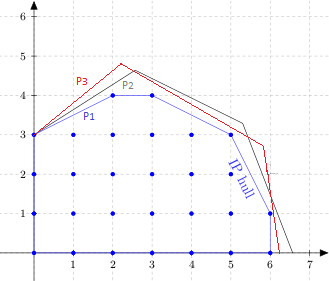
\includegraphics[scale=1.0]{figures/linearForm3.png}
\caption{Different linear formulations}
\label{fig:linearForm}
\end{figure}

Following are some useful definitions for the subject.

\paragraph{Definition}
A subset of $\mathbb{R}^{n}$ described by a finite set of linear constraints $P=\{x \in \mathbb{R}^{n}: Ax \le b\}$ is a \textit{polyhedron}.

\paragraph{Definition}
A polyhedron $P \subseteq \mathbb{R}^{n+p}$ is a \textit{formulation} for a set $X \subseteq \mathbb{Z}^{n} \times \mathbb{R}^{p}$ if and only if $X = P \cup (\mathbb{Z}^{n} \times \mathbb{R}^{p})$.

\vspace{7 mm}

Although all three formulations in figure ~\ref{fig:linearForm} are valid for definition of subset $X$, the formulation $P_{1}$ is ideal, because solving a linear program over $P_{1}$ leads to an optimal solution lying at an extreme point. Since each extreme point of $P_{1}$ is integer, it follows that the integer program is solved.

Generally speaking, given a set $X \subseteq \mathbb{R}^n$ and two formulations $P_{1}$ and $P_{2}$ for $X$, $P_{1}$ is a better formulation than $P_{2}$ if $P_{1} \subset P_{2}$. Formulation $P_{1}$ is said to be \textit{tighter} than $P_{2}$.



%%%%%%%%%%%%%%%%%%%%%%%%%%%%%%%
\subsection{Optimality and relaxation}

Regardless of the method used in the search for the optimal solution $x^*$ of an integer program, some stopping criteria is needed in the algorithm, which is equivalent to prove that a given point $x^*$ is optimal.
A pretty intuitive way is to obtain lower and upper bounds for the objective function value of the optimal solution. Hence, given an IP $$z = max\{c(x): x \in X \subseteq \mathbb{Z}^n\},$$ any algorithm will construct a decreasing sequence $$\overline{z_{1}} \ge \overline{z_{2}} \ge \ldots \overline{z_{s}} \ge z$$ of upper bounds, and an increasing sequence $$\underline{z_{1}} \le \underline{z_{2}} \le \underline{z_{t}} \le \ldots z$$ of lower bounds, and stop when $z_{s} - z_{t}$ is small enough.

Considering a maximization problem, any feasible solution provides a lower bound, also known as primal bounds. Finding upper bounds, known as dual bounds, is a different challenge. The main approach is by \q{relaxation}, the idea being to replace a difficult max (min) $IP$ by a simpler optimization problem whose optimal value is at least as large (small) as $z$.

\paragraph{Definition}
A problem (RP) $z^R = max\{f(x): x \in T \subseteq \mathbb{R}^n\}$ is a relaxation of (IP) $z = max\{c(x): x \in X \subseteq R^n\}$ if:
\begin{enumerate}
\item $X \subseteq T$, and
\item $f(x) \ge c(x)$ for all $x \in X$
\end{enumerate}

\paragraph{Proposition}
If RP is a relaxation of IP, then $z^R \ge z$.

%%%%%%%%%%%%%%
\subsubsection{Linear programming relaxation}

One way of relaxing an integer program is to enlarge the set of feasible solutions so that one optimizes over a larger set. For example, at figure ~\ref{fig:linearForm} all the three formulations $P_{1}$, $P_{2}$ and $P_{3}$ are relaxations of the original problem if we ignore the integrality constraints.

\paragraph{Definition}
For the integer program $max\{c(x): x \in P \cup \mathbb{Z}^n\}$ with formulation $P = \{x \in \mathbb{R}^{n}_{+}: Ax \le b\}$, the \textit{linear programming relaxation} is the linear program $z^{LP} = max\{cx: x \in P\}$.

However, the more the feasible solution space is enlarged, the more different the relaxed problem becomes from the original problem, which can lead to more distinct optimal solutions values for both problems. When using linear relaxations for obtaining dual bounds, this is very relevant. The more relaxed in the objective function direction is the formulation, the more distant from the actual optimal solution value will be the upper bound obtained, as illustrated in figure ~\ref{fig:objDirection}. In general, the tighter is the relaxation, the better.

\begin{figure}[h]
\centering
\hfill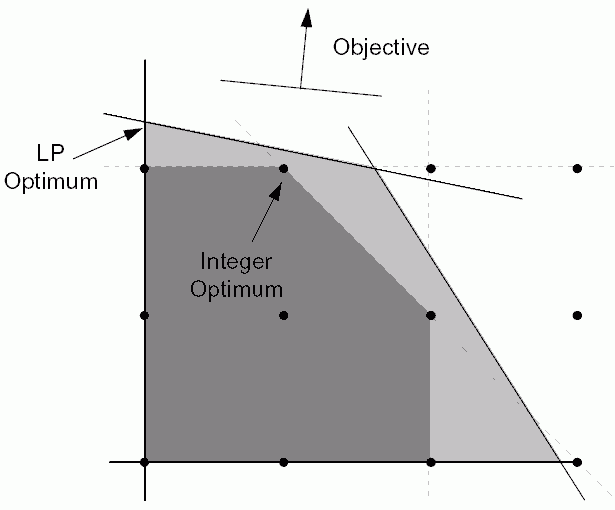
\includegraphics[scale=0.6]{figures/linearForm2.png}
\caption{Linear relaxation in the direction of objective function}
\label{fig:objDirection}
\end{figure}

Notice, though, that for a relaxation of a IP to provide an upper bound, it must be solved to optimality.

%%%%%%%%%%%%%%
\subsubsection{Duality}

Another way of finding dual bounds is through duality properties. Consider the previously introduced linear program given by \eqref{eq:LP}, called \textit{primal} problem, the following problem is referred as its \textit{dual} problem.

\begin{subequations}
\label{eq:Dual}
\begin{align}
   \mbox{Minimize } & u \cdot b
								\\ & u \cdot A \ge c
								\\ & u \in \mathbb{R}^{m}_{+}
\end{align}
\end{subequations}

Every linear program has an associated dual problem. The value of \textit{any} dual feasible solution provides an upper bound on the primal objective function value, which makes it an advantage compared to the linear relaxation. A linear programming relaxation immediately leads to a dual problem, which can then be used to obtaining dual bounds.


%%%%%%%%%%%%%%%%%%%%%%%%%%%%%%%
\subsection{Integrality gap}

Linear programming relaxation is thus a standard technique for designing approximation algorithms for optimization problems. Since such relaxation removes variables' integrality constraints, the optimal value for the relaxed maximization problem is necessarily greater than or equal to the optimal value for the original problem. The integrality gap is the maximum ratio between the solution quality of the integer program and of its relaxation. It essentially represents the inherent limits of a particular linear relaxation in approximating an integer program. Thus, the more the integral solution is improved, the smaller becomes the integrality gap.


%%%%%%%%%%%%%%%%%%%%%%%%%%%%%%%
\subsection{Branch and Bound}

Branch and bound is an implicit enumeration method for feasible solutions of combinatorial problems. Complete enumeration is inefficient and not applicable for real optimization problems, but using some knowledge on partition strategies of the problem it is possible to make intelligent decisions on whether it is necessary to explore a set of new potential solutions or about which set of potential solutions is more promising.

The \q{branch} word refers to the partitioning process of the problem and the \q{bound} refers to the decision of not exploring some set of possible new solutions (branch), avoiding exhaustive search. The bounding decisions use information of dual bounds to construct evidences of optimality and thus to eliminate branches that have proved to be unsuccessful.

Basically, for an integer linear program, the problem is decomposed and organized as a tree where each node is a subset of the solution space and a branch on that node splits the subset into mutually exclusive subsubsets. Each resulting subsubset in the partition is represented by a child of the original node. An algorithm based on linear programming is then used for calculating a dual bound on the cost of any solution in a given subset.

For further information about the branch and bound process and its strategies, see \cite{Wolsey98} and \cite{Papa98}.


%%%%%%%%%%%%%%%%%%%%%%%%%%%%%%%
\subsection{MIP Solver}

For decades limitation of computational resources was an obstacle to the development of efficient mathematical programming solvers. Since the early 90's though, advances in technology and algorithm design have allowed significant improvements in the area.

For mathematical programming there are some well-known solvers available. The most popular commercial software for optimization of (mixed integer) linear programming are IBM ILOG CPLEX Optimization Studio \fixme{conferir cplex} (\cite{Cplex}), also simply known as Cplex, and Gurobi Optimizer (\cite{Gurobi}). Both are accessible from several programming languages. CPLEX Optimization was founded in 1987, was acquired by ILOG in 1997, which was subsequently acquired by IBM in January 2009. Gurobi Optimizer was founded in 2009 by a team previously responsible for Cplex development.


This work was developed using \textit{Gurobi Optimizer version 6.0} for solving the mathematical models.



%%%%%%%%%%%%%%%%%%%%%%%%%%%%%%%%%%%%%%%%%%%%%%%%%%%%%%%%%%%%%%%%%%%%%%%%%%%%%%%%%%
%%%%%%%%%%%%%%%%%%%%%%%%%%%%%    MATH FORMULATION     %%%%%%%%%%%%%%%%%%%%%%%%%%%%
%%%%%%%%%%%%%%%%%%%%%%%%%%%%%%%%%%%%%%%%%%%%%%%%%%%%%%%%%%%%%%%%%%%%%%%%%%%%%%%%%%

\section{IP - Assignment Formulation for the Timetabling Problem}
\label{sec:mathForm}

The general process of formulating an integer program can be organized in three steps:

\begin{enumerate}
\item Define what appear to be the necessary variables.
\item Use these variables to define a set of constraints so that the feasible points correspond to feasible solutions to the problem.
\item Use these variables to define the objective function.
\end{enumerate}

Usually the need of auxiliary variables arises while formulating constraints, which gives an iterative feature to the process until a consistent model is reached.

Next subsections introduce the notation used in the mathematical model, which includes data sets, general data and model variables, and the formulation, which includes a multi-objective function and all constraints.

%%%%%%%%%%%%%%%%%%%%%%%%%%%%%%%%%%%%%%%%%%%%%%%%%%%%%%%%%%%%%%%%%%%%%%%%%%%%%%%%%%

\subsection{Notation}

%%%%%%%%%%%%%%%%%%%%%%%%%%%%%%%%%%%%%%%%%%
\subsubsection{Sets}

\begin{itemize}
\item $Al$ - Set of students. Elements of $Al$ are called $a$.
\item $C$ - Set of majors. Elements of $C$ are called $c$.
\item $D$ - Set of courses. Elements of $D$ are called $d$.
\item $Dm$ - Set of courses for which lessons are shareable between different classes, that is, lessons can be \textit{merged}. Elements of $D$ are called $d$.
\item $D_{a}$ - Set of courses required by student $a$.
\item $H$ - Set of time slots. Elements of $H$ are called $h$.
\item $H_{f}$ - Set of time slots of session of day $f$. Elements are called $h$.
\item $I_{d}$ - Set of sections of a course $d$. Elements of $I_{d}$ are called $i$.
\item $O$ - Set of majors offers. Elements of $O$ are called $oft$.
\item $U$ - Set of blocks. Elements of $U$ are called $u$.
\item $S_{u}$ - Set of classrooms of block $u$. Elements of $S_{u}$ are called $s$.
\item $T$ - Set of weekdays. Elements of $T$ are called $t$.
\item $U$ - Set of blocks. Elements of $U$ are called $u$.
\item $SL$ - Set of calenders. Elements of $SL$ are called $sl$.
\item $P$ - Set of all professors. Elements of $P$ are called $p$.
\item $P_{prior}$ - Set of all professors with some priority $prior$. Elements of $P$ are called $p$.
\end{itemize}

%%%%%%%%%%%%%%%%%%%%%%%%%%%%%%%%%%%%%%%%%%
\subsubsection{Model Data}

\begin{itemize}
\item $Cap_{s}$ - Capacity of classroom $s$.
\item $nCreds_{d}$ - Total of credits of course $d$.
\item $duration_{h}$ - Total of minutes of time slot $h$.
\item $duration_{hi,hf}$ - Total of minutes from the beginning of time slot $hi$ to the end of time slot $hf$.
\item $M$ - called \q{big M}, it is a large enough value that depends on the constraint it is applied to.
\item $N_{d,k,t}$ - number of credits for course $d$ at day $t$ of credits split rule $k$.
\item $NCH_{d,hi,hf}$ - number of credits for course $d$ from time slot $hi$ to time slot $hf$.
\item $MinSize$ - minimum number of students required for offering a class.
\item $delta_{t,f}$ - maximum of idle time allowed at phase $f$ of day $t$ for a professor. Used only for gap-constraints, usually is the average sum of intervals at phase $f$ of day $t$ of calenders.
\item $pv$ - Unique virtual professor, to be used whenever the set of real professors is not enough for demand satisfaction.
\item $MinCredsDia_{a,t}$ - minimum number of credits expected for student $a$ at day $t$.
\item $MaxNrCredsDay_{p,t}$ - maximum number of credits available at day $t$ of professor $p$.
\item $Time_{u1,u2}$ - minimum number of minutes necessary for moving between blocks $u1 \in U$ and $u2 \in U$.
\item $MaxGapBetweenSessions$ - maximum idle interval between 2 consecutive day sessions that a professor is assigned to. It is used to avoid situations like a professor being assigned to a class early in the morning and then another just late in the afternoon, with a big idle inbetween interval. A reasonable value is around 170 minutes.
\end{itemize}

%%%%%%%%%%%%%%%%%%%%%%%%%%%%%%%%%%%%%%%%%%
\subsubsection{Variables}

All possible variables used in the model are following described. The need of some of them depends on considering or not some constraints, in the sense that the more restrictions and requirements exist, the more auxiliary variables are need.

\begin{itemize}
\item $v_{a,i,d,s,t,hi,hf}$ - binary variable, indicates if student $a$ is assigned to a class of section $i$ of course $d$, at classroom $s$, from time slot $hi$ to time slot $hf$ of day $t$. 
\item $x_{i,d,u,s,hi,hf,t}$ - binary variable, indicates if section $i$ of course $d$ is assigned to classroom $s$ from time slot $hi$ to time slot $hf$ of day $t$. 
\item $z_{i,d}$ - binary variable, indicates if section $i$ of course $d$ is offered. 
\item $o_{i,d,s}$ - binary variable, indicates if section $i$ of course $d$ is offered at classroom $s$. 
\item $fd_{d,a}$ - binary slack variable, indicates if student $a$ has his request for course $d$ not satisfied.
\item $m_{d,i,k}$ - binary variable, indicates if a credits split rule $k$ was chosen for section $i$ of course $d$.
\item $s_{i,d,a}$ - binary variable, indicates if student $a$ is assigned to section $i$ of course $d$.
\item $k_{p,i,d,u,h,t}$ - binary variable, indicates if professor $p$ teaches to section $i$ of course $d$ at block $u$ at time slot $h$ and day $t$.
\item $y_{p,i,d}$ - binary variable, indicates if professor $p$ is assigned to section $i$ of course $d$.
\item $hip_{p,t,f}$ - integer variable, indicates the time in minutes of the first time slot assigned to professor $p$ at session $f$ of day $t$. For example, if the first class assigned to $p$ on $t=Monday$ and $f=morning$ starts at 9:30 am, then $hip_{p,t,f}=9\cdot 60 + 30 = 570$.
\item $hfp_{p,t,f}$ - integer variable, indicates the time in minutes of the end of the last time slot assigned to professor $p$ at session $f$ of day $t$.
\item $fpgap_{p,t,f}$ - integer slack variable, indicates the gap in session $f$ of day $t$ of professor $p$'s schedule.
\item $fcad_{a,t}$ - integer slack variable, indicates the number of credits bellow the expected assigned to student $a$ at day $t$.
\item $begin_{a,t,h}$ - binary variable, indicates if first class of student $a$ at day $t$ begin at time $h$.
\item $end_{a,t,h}$ - binary variable, indicates if last class of student $a$ at day $t$ begin at time $h$.
\item $at_{a,t}$ - binary variable, indicates if student $a$ has classes at day $t$.
\item $uu_{p,t,u}$ - binary variable, indicates if professor $p$ has classes at day $t$ in block $u$.
\item $desloc_{p,t,u1,u2}$ - binary variable, indicates whether professor $p$ has classes at day $t$ in block $u1$ and in block $u2$. In practice, it identifies that at least one displacement is made between the both blocks in the day.
\item $ptf_{p,t,f}$ - binary variable, indicates if professor $p$ has classes at session $f$ of day $t$.
\item $pt_{p,t}$ - binary variable, indicates if professor $p$ has classes at day $t$.


\end{itemize}


%%%%%%%%%%%%%%%%%%%%%%%%%%%%%%%%%%%%%%%%%%%%%%%%%%%%%%%%%%%%%%%%%%%%%%%%%%%%%%%%%%
%%%%%%%%%%%%%%%%%%%%%%%%%%%%%%%%%%%%%%%%%%%%%%%%%%%%%%%%%%%%%%%%%%%%%%%%%%%%%%%%%%

\subsection{Formulation}


\subsubsection{Objective function}

The following general objective function includes all possible minimization goals, with their subjective weights to be decided according to the scenario or the user preferences. Further alternatives of how to handle disparate goals are discussed at section ~\ref{sec:goal}.

$$
\begin{array}{rl}
   \mbox{MIN} &
			\lambda \cdot \sum\limits_{a \in A}\sum\limits_{d \in D} \cdot fd_{d,a}
      \\
      &
       + \beta \cdot \sum\limits_{a \in A} \sum\limits_{t \in T} fcad_{a,t}
      \\
      &      
      + \epsilon \cdot \sum\limits_{p \in P} \sum\limits_{t \in T} \sum\limits_{f \in F} fpgap_{p,t,f}
			\\
			&
			+ \sigma \cdot \sum\limits_{p \in P} \sum\limits_{t \in T} \sum\limits_{u1 \in U} \sum\limits_{u2 \in U} Time_{u1,u2} \cdot desloc_{p,t,u1,u2}
      \\
      &
      + \gamma \cdot \sum\limits_{i \in I_{d}} \sum\limits_{d \in D} y_{pv,i,d}
      \\
      &
      + \alpha \cdot \sum\limits_{p \in P} \sum\limits_{t \in T} pt_{p,t}
      \\
      &
      + \alpha \cdot \sum\limits_{p \in P} \sum\limits_{t \in T} \sum\limits_{f \in F} ptf_{p,t,f}
      
\end{array}
$$


%%%%%%%%%%%%%%%%%%%%%%%%%%%%%%%%%%%%%%%%%%%%%%%%%%%%%%%%%%%%%%%%%%%%%%%%%%%%%%%%%%
%%%%%%%%%%%%%%%%%%%%%%%%%%%%%%%%%%%%%%%%%%%%%%%%%%%%%%%%%%%%%%%%%%%%%%%%%%%%%%%%%%


\subsubsection{Assigns 'v' to 'x' and ensures classroom capacity}
\begin{eqnarray}
\sum\limits_{a \in A} v_{a,i,d,s,t,hi,hf}  \le Cap_{s} \cdot x_{i,d,s,t,hi,hf} \nonumber \qquad 
\\
\forall d \in D \quad
\forall i \in I_{d} \quad 
\forall s \in S \quad
\forall t \in T \quad 
\forall hi \in H \quad 
\forall hf \in H \nonumber
\end{eqnarray}

\subsubsection{Assigns the classroom of a section to variable 'o'}
\begin{eqnarray}
M \cdot o_{i,d,s}  \geq \sum\limits_{t \in T}\sum\limits_{hi \in H}\sum\limits_{hf \in H} x_{i,d,s,t,hi,hf}  \nonumber \qquad 
\\
\forall d \in D \quad
\forall i \in I_{d} \quad
\forall u \in U \quad
\forall s \in S_{u} \nonumber
\end{eqnarray}

\subsubsection{Ensures single classroom per course section}
\begin{eqnarray}
\sum\limits_{u \in U} \sum\limits_{s \in S_{u}} o_{i,d,s} = z_{i,d}  \nonumber \qquad 
\forall d \in D \quad
\forall i \in I_{d} \quad
\end{eqnarray}

\subsubsection{No overlapping in classroom's timetable}
\begin{eqnarray}
\sum\limits_{i \in I_{d}} \sum\limits_{d \in D} \sum\limits_{hi \in H_{d}} \sum_{\substack {hf \in H_{d} \\ hi\le hf}} x_{i,d,s,t,hi,hf}  \leq  1  \nonumber \qquad 
\\
\forall u \in U \quad
\forall s \in S_{u} \quad
\forall t \in T \quad
\forall h \in H \quad (hi,hf)\text{ overlaps }h \nonumber
\end{eqnarray}

\subsubsection{Tries to satisfy each student requirement}
\begin{eqnarray}
\sum\limits_{i \in I_{d}} s_{i,d,a} + fd_{d,a} = 1  \nonumber \qquad 
\forall a \in Al \quad
\forall d \in D_{a}
\end{eqnarray}

\subsubsection{Assigns student's course section to lessons, while ensures course section's total number of credits}
\begin{eqnarray}
nCreds_{d} \cdot s_{i,d,a} = \sum\limits_{s \in S}\sum\limits_{t \in T}\sum\limits_{hi \in H}\sum\limits_{hf \in H} NHC_{d,hi,hf} \cdot v_{a,i,d,s,t,hi,hf} \nonumber \qquad 
\forall a \in A \quad
\forall i \in I_{d} \quad
\forall d \in D_{a}
\end{eqnarray}

\subsubsection{Links variables x and variable z, while ensures course section's total number of credits}
\begin{eqnarray}
\sum\limits_{s \in S}\sum\limits_{t \in T}\sum\limits_{hi \in H}\sum\limits_{hf \in H} NHC_{d,hi,hf} \cdot x_{i,d,s,t,hi,hf} = nCreds_{d} \cdot z_{i,d} \nonumber \qquad
\forall i \in I_{d} \quad
\forall d \in D \quad
\end{eqnarray}

\subsubsection{Avoids classes overlapping at student timetable}
\begin{eqnarray}
\sum\limits_{u \in U} \sum\limits_{s \in S_{u}} \sum\limits_{i \in I_{d}} \sum\limits_{d \in D_{a}} \sum\limits_{hi \in H_{d}} \sum_{\substack {hf \in H_{d} \\ hi\le hf \\ (hi,hf)\mbox{ overlaps }h}} v_{a,i,d,s,hi,hf,t}  \leq  1  \nonumber \qquad 
\\
\forall a \in A \quad
\forall t \in T \quad
\forall h \in H_{d} \nonumber
\end{eqnarray}

\subsubsection{Single lesson for each course section per day}
\begin{eqnarray}
\sum\limits_{u \in U} \sum\limits_{s \in S_{u}} \sum\limits_{hi \in H_{d}} \sum_{\substack {hf \in H_{d} \\ hi\le hf}} x_{i,d,s,hi,hf,t}  \leq  1  \nonumber \qquad 
\forall d \in D \quad
\forall i \in I_{d} \quad
\forall t \in T 
\end{eqnarray}


%%%%%%%%%%%%%%%%%%%%%%%%%%%%%%%%%%%%%%%%%%%%%%%%%%%%%%%%%%%
% 		EXPECTED NUMBER OF CREDITS FOR EACH STUDENT PER DAY

\subsubsection{Try to ensure the expected number of credits for each student per day}
\begin{eqnarray}
\sum\limits_{i \in I_{d}} \sum\limits_{d \in D_{a}} \sum\limits_{s\in S} \sum\limits_{hi\in H} \sum\limits_{hf\in H} nCreds_{d} \cdot v_{a,i,d,s,t,hi,hf} + fcad_{a,t} \ge MinCredsDia_{a,t} \nonumber \qquad
\forall a \in A \quad
\forall t \in T
\end{eqnarray}


%%%%%%%%%%%%%%%%%%%%%%%%%%%%%%%%%%%%%%%%%%%%%%%%%%%%%%%%%%%
% 					CREDITS SPLIT RULES
\subsubsection{Credits split rules}

\paragraph{Credits split rule for each course section}
\begin{eqnarray}
\sum\limits_{u \in U} \sum\limits_{s \in S_{u}} \sum\limits_{hi \in H_{d}} \sum_{\substack {hf \in H_{d} \\ hi\le hf}}
 NCH_{d,hi,hf} \cdot x_{i,d,u,s,hi,hf,t} = \sum\limits_{k \in K_{d}}N_{d,k,t} \cdot m_{d,i,k} \nonumber \qquad 
\\
\forall d \in D \quad
\forall i \in I_{d} \quad
\forall t \in T \nonumber
\end{eqnarray}

\paragraph{Single credits split rule for each course section}
\begin{eqnarray}
\sum\limits_{k \in K_{d}} m_{d,i,k} = z_{i,d} \nonumber \qquad 
\forall d \in D \quad
\forall i \in I_{d}
\end{eqnarray}


%%%%%%%%%%%%%%%%%%%%%%%%%%%%%%%%%%%%%%%%%%%%%%%%%%%%%%%%%%%
% 				GAPS IN STUDENT'S TIMETABLE
\subsubsection{Student's gaps prohibition}
\label{constrStudentGap}

Following, auxiliary variables necessary for preventing gaps in student's timetable are consistently set.

\paragraph{Sets if student $a$ has classes at day $t$ (variable $at_{a,t}$)}
\begin{eqnarray}
M \cdot at_{a,t} \ge \sum\limits_{i \in I_{d}} \sum\limits_{d \in D_{a}} \sum\limits_{u \in U} \sum\limits_{s \in S_{u}} \sum\limits_{hi \in H_{d}} \sum_{\substack {hf \in H_{d} \\ hi\le hf}} v_{a,i,d,u,s,hi,hf,t} \nonumber \qquad 
\forall a \in A \quad
\forall t \in T
\end{eqnarray}

\paragraph{Sets beginning time of classes for student $a$ at day $t$ (variable $begin_{a,t,h}$)}
\begin{eqnarray}
begin_{a,t,h} = \sum\limits_{v} v_{a,t,hi} - \sum\limits_{h'\le h} begin_{a,t,h'} + \sum\limits_{h'\le h} end_{a,t,h'} \nonumber \qquad
\forall a \in A \quad
\forall t \in T \quad
\forall h \in H
\end{eqnarray}

\paragraph{Sets ending time of classes for student $a$ at day $t$ (variable $end_{a,t,h}$)}
\begin{eqnarray}
end_{a,t,h} = \sum\limits_{v} v_{a,t,hi} - \sum\limits_{h'\ge h} end_{a,t,h'} + \sum\limits_{h'\ge h} begin_{a,t,h'} \nonumber \qquad
\forall a \in A \quad
\forall t \in T \quad
\forall h \in H
\end{eqnarray}

\paragraph{Uniqueness of student's last class of the day}
\begin{eqnarray}
\sum\limits_{h\in H} end_{a,t,h} = at_{a,t} \nonumber \qquad
\forall a \in A \quad
\forall t \in T
\end{eqnarray}

\paragraph{Uniqueness of student's first class of the day}
\begin{eqnarray}
\sum\limits_{h\in H} begin_{a,t,h} = at_{a,t} \nonumber \qquad
\forall a \in A \quad
\forall t \in T
\end{eqnarray}


Next, gaps in student timetable are prevented. Unlike professors similar restriction, students can not have idle times, and therefore these are hard constraints and there are no slack variables.

\paragraph{Prohibits gap in student timetable}
\begin{eqnarray}
\sum\limits_{i\in I_{d}} \sum\limits_{d\in D} \sum\limits_{s\in S} \sum\limits_{hf\in H} v_{a,i,d,s,t,hi+,hf} = 
\sum\limits_{i\in I_{d}} \sum\limits_{d\in D} \sum\limits_{s\in S} \sum\limits_{hf\in H} v_{a,i,d,s,t,hi-,hf} - end_{a,t,hi-} + begin_{a,t,hi+} \nonumber \qquad
\\
\forall a \in A \quad
\forall t \in T \quad
\forall hi+ \in H \quad hi- \in H \mbox{ s.t. hi- + 1 = hi+} \nonumber
\end{eqnarray}


%%%%%%%%%%%%%%%%%%%%%%%%%%%%%%%%%%%%%%%%%%%%%%%%%%%%%%%%%%%
% 					PROFESSORS ASSIGNMENT
\subsubsection{Professors assignment}

The following constraints, responsible for assigning professors to classes, involve both real professors and the virtual teaching resource $pv$.

\paragraph{No overlapping in professor's timetable}
\begin{eqnarray}
\sum_{ \substack {dti,dtf \in Dt \\ dt \in [dti,dtf)} } \sum\limits_{i \in I_{d}} \sum\limits_{d \in D} \sum\limits_{u \in U} k_{p,i,d,u,t,dti,dtf} \le 1 \nonumber \qquad
\forall p \in P \cup \{pv\} \quad
\forall t \in T \quad
\forall dt \in Dt
\end{eqnarray}

\paragraph{Assigns professor to class (sets variable k)}
% Part 1
\begin{eqnarray}
\sum_{ \substack {hi,hf \in H \\ dti \in [hi,hf)} } \sum\limits_{s\in S_{u}} x_{i,d,s,t,hi,hf} \le k_{p,i,d,u,t,dti} + ( 1 - y_{p,i,d} ) \nonumber \qquad
\\
\forall i \in I \quad
\forall d \in D \quad
\forall u \in U \quad
\forall p \in P \cup \{pv\} \quad
\forall t \in T \quad
\forall dti \in Dt \nonumber
\end{eqnarray}
% Part 2
\begin{eqnarray}
\sum_{ \substack {hi,hf \in H \\ dti \in [hi,hf)} } \sum\limits_{s\in S} x_{i,d,s,t,hi,hf} \le \sum\limits_{u\in U} \sum\limits_{p \in P \cup \{pv\}} k_{p,i,d,u,t,dti} \nonumber \qquad
\\
\forall i \in I \quad
\forall d \in D \quad
\forall t \in T \quad
\forall dti \in Dt \nonumber
\end{eqnarray}
	
\paragraph{Assigns professor to class (sets variable y)}
\begin{eqnarray}
\sum\limits_{u \in U} \sum\limits_{t \in T} \sum\limits_{h \in H} k_{p,i,d,u,t,h} = nCreds_{d} \cdot y_{p,i,d} \nonumber \qquad
\forall i \in I \quad
\forall d \in D \quad
\forall p \in P \cup \{pv\}
\end{eqnarray}	
	
\paragraph{Assigns a single professor to each course section}
\begin{eqnarray}
\sum\limits_{p\in P \cup \{pv\}} y_{p,i,d} = z_{i,d} \nonumber \qquad
\forall i \in I \quad
\forall d \in D
\end{eqnarray}	


%%%%%%%%%%%%%%%%%%%%%%%%%%%%%%%%%%%%%%%%%%%%%%%%%%%%%%%%%%%
%						PROFESSOR DISPLACEMENT
\subsubsection{Professor's displacement}
\label{constrProfessorDisplac}

Here quality constraints related to displacement of real professors along the week and in a day are considered.


\paragraph{Ensures enough time for displacement between blocks in the same day}
\begin{eqnarray}
\sum\limits_{i \in I_{d}} \sum\limits_{d \in D} k_{p,i,d,u1,t,h1} + \sum\limits_{i\in I_{d}} \sum\limits_{d \in D} k_{p,i,d,u2,t,h2} \le 1 \nonumber
\\
\forall p \in P \quad
\forall t \in T \quad
\forall u1 \in U \quad
\forall u2 \in U \quad
\forall h1 \in H \quad
\forall h2 \in H \nonumber
\end{eqnarray}	
\textit{s.t. time between ending of h1 and beginning of h2 is less than displacement time between u1 and u2}.

\paragraph{Ensures the maximum of 1 displacement for each professor in the same day}
\begin{eqnarray}
\sum\limits_{i\in I_{d}} \sum\limits_{d \in D} k_{p,i,d,u1,t,h1} + \sum\limits_{i\in I_{d}} \sum\limits_{d \in D} k_{p,i,d,u2,t,h2} + \sum\limits_{i\in I_{d}} \sum\limits_{d \in D} k_{p,i,d,u3,t,h3} \le 2 \nonumber
\\
\forall p \in P \quad
\forall t \in T \quad
\forall u2 \in U \quad
\forall h2 \in H \nonumber
\\
\mbox{s.t. }u1 \neq u2 \qquad u3 \neq u2 \qquad h1<h2 \qquad h3>h2 \nonumber
\end{eqnarray}

\paragraph{Identifies if the professor teaches in a block at the day}
\begin{eqnarray}
\sum\limits_{i\in I_{d}} \sum\limits_{d \in D} \sum\limits_{h \in H} k_{p,i,d,u,t,h} \le MaxNrCredsDay_{p,t} \cdot uu_{p,t,u} \nonumber \qquad
\\
\forall p \in P \quad
\forall t \in T \quad
\forall u \in U \quad \nonumber
\end{eqnarray}

\paragraph{Constraints the maximum number of blocks assigned to the professor at the day}
\begin{eqnarray}
\sum\limits_{u \in U} uu_{p,t,u} \le 2 \nonumber \qquad
\forall p \in P \quad
\forall t \in T \quad \nonumber
\end{eqnarray}

\paragraph{Identifies displacements in the day of the professor}
\begin{eqnarray}
uu_{p,t,u1} + uu_{p,t,u2} \le 1 + desloc_{p,t,u1,u2} \nonumber \qquad
\\
\forall p \in P \quad
\forall t \in T \quad
\forall u1 \in U \quad
\forall u2 \in U \quad \mbox{s.t. }u1 \neq u2 \nonumber
\end{eqnarray}


\paragraph{Limits the maximum of 2 big displacements for each professor along the week}
\begin{eqnarray}
\sum\limits_{t \in T} \sum\limits_{u1 \in U} \sum_{\substack {u2 \in U \\ \norm{u1 u2} \ge 50}} desloc_{p,t,u1,u2} \le 2 \nonumber \qquad
\forall p \in P \quad \nonumber
\end{eqnarray}



%%%%%%%%%%%%%%%%%%%%%%%%%%%%%%%%%%%%%%%%%%%%%%%%%%%%%%%%%%%
%						GAPS IN PROFESSOR'S TIMETABLE									% 							 
\subsubsection{Professor's gaps avoidance}
\label{constrProfessorGap}

Next, variables $hip_{p,t,f}$ and $hfp_{p,t,f}$ are set. We draw attention to the fact of these variables being strictly set, i.e., less and greater inequality constraints are used per variable, resulting in an implicit equality constraint. Consequently, they do not depend on an objective function, which is important when it has conflicting goals. \fixme{Exemplify!} \fixme{exception when the professor is not assigned at the day}

\paragraph{Sets variable $hip_{p,t,f}$}
\begin{eqnarray}
hip_{p,t,f} \geq m(dt) \cdot ( 1 - \sum\limits_{k \in K_{dti<dt}} k_{p,t,dti} ) \nonumber \qquad
\forall p \in P \quad
\forall t \in T \quad
\forall f \in F \quad
\forall dt \in Dt_{f}
\end{eqnarray}
\begin{eqnarray}
hip_{p,t,f} \leq m(dt) + M \cdot ( 1 - \sum\limits_{k} k_{p,t,dti} ) \nonumber \qquad
\forall p \in P \quad
\forall t \in T \quad
\forall f \in F \quad
\forall dti \in Dt_{f}
\end{eqnarray}

\paragraph{Sets variable $hfp_{p,t,f}$}
\begin{eqnarray}
hfp_{p,t,f} \geq \sum\limits_{k} m(dt) \cdot k_{p,t,dtf} \nonumber \qquad
\forall p \in P \quad
\forall t \in T \quad
\forall f \in F \quad
\forall dtf \in Dt_{f}
\end{eqnarray}
\begin{eqnarray}
hfp_{p,t,f} \leq m(dt) + M \cdot ( \sum\limits_{k \in K_{dtf>dt}} k_{p,t,dtf} ) \nonumber \qquad
\forall p \in P \quad
\forall t \in T \quad
\forall f \in F \quad
\forall dt \in Dt_{f}
\end{eqnarray}

Next, gaps in professor timetable are controlled. The usage of the slack variable $fpgap_{p,t,f}$ indicates the amount of idle time in session $f$ of day $t$ for professor $p$. The reduce of professors idle time is achieved through minimization of these slack variables in objective function.

\paragraph{Prohibits gap in each session of day in professor timetable}
\begin{eqnarray}
\sum\limits_{k \in K_{h \in H_{f}}} duration_{h} \cdot k_{p,t,h} + delta_{f,t} + fpgap_{p,t,f} \geq hfp_{p,t,f} - hip_{p,t,f} \nonumber \qquad
\\
\forall p \in P \quad
\forall t \in T \quad
\forall f \in F \quad \nonumber
\end{eqnarray}



%%%%%%%%%%%%%%%%%%%%%%%%%%%%%%%%%%%%%%%%%%%%%%%%%%%%%%%%%%%
%						COMPACTING PROFESSOR'S TIMETABLE							% 							 
\subsubsection{Professor's timetable compactness}
\label{constrProfCompact}

Besides constraints introduced at ~\ref{constrProfessorGap}, specific for avoiding gaps in each session of a professor's day, here further quality constraints related to compactness of real professors' timetable along the week and in a day are considered.


\paragraph{Sets if a session of day is assigned for the professor}
\begin{eqnarray}
M \cdot ptf_{p,t,f} \ge \sum\limits_{d \in D}\sum\limits_{i \in I_{d}}\sum\limits_{u \in U}\sum\limits_{h \in H_{f}} k_{p,i,d,u,t,h} \nonumber \qquad
\\
\forall p \in P \quad
\forall T \in T \quad
\forall f \in F \nonumber
\end{eqnarray}

\paragraph{Sets the number of days of the week assigned to each professor}
\begin{eqnarray}
M \cdot pt_{p,t} \ge \sum\limits_{f \in F} ptf_{p,t,f} \nonumber \qquad
\forall p \in P \quad
\forall t \in T \nonumber
\end{eqnarray}

\paragraph{Prohibits big gaps between assigned sessions of the day}
\begin{eqnarray}
hip_{p,t,f} - hfp_{p,t,f-1} \le (MaxGapBetweenSessions + M \cdot(2 - ptf_{p,t,f} - ptf_{p,t,f-1}))  \nonumber \qquad
\\
\forall p \in P \quad
\forall t \in T \quad
\forall f \in F \quad \nonumber
\end{eqnarray}



%%%%%%%%%%%%%%%%%%%%%%%%%%%%%%%%%%%%%%%%%%%%%%%%%%%%%%%%%%%%%%%%%%%%%%%%%%%%%%%%%%%%%%%%%%

\chapter{Solving Strategies}
\label{chap:strategies}

This chapter describes and compares different strategies and approaches used and tested during solver development.


%%%%%%%%%%%%%%%%%%%%%%%%%%%%%%%%%%%%%%%%%%%%%%%%%%%%%%%%%%%%%%%%%%%%%%%%%%%%%%%%%%
\section{Goal programming}

Just as in any other kind of problem, the feasibility of a linear model for a timetabling problem depends utterly on data set. In general, there is no guarantee that all demanded requirements can be satisfied with the specified available resources, even because usually there are several and conflicting objectives. Therefore, specially in a commercial solver, it is important to treat some idealistic hard constraints as highest priority soft constraints, otherwise the solver could frequently generate an infeasible model.

In real life it is useless for an educational institution to have a solution that satisfies all demands of students for courses, but which does not respect some important quality requirements. Bearing this in mind, in addition to the feasibility issue, the model presented at this work, unlike most authors, does not consider demand satisfaction as a hard constraint. Essential quality requirements are modeled as hard constraints though, and demand satisfaction is treated as the highest priority objective, followed by some further goals.

While it is not easy to embody quality into the modeling process, it can be even more difficult to quantify it. A \textbf{multi-objective function} unifies disparate goals of the model in a single weighted sum of preferences. Such approach, although simpler, depends on very subjective choice of weights and is not always consistently reliable, specially when objectives are mutually conflicting.

An alternative approach is using a priority line for the different goals. According to the institution preferences, one optimizes the problem in a sequence of steps, where each step is responsible for a goal, from the most to the least important. For each step a different and specific objective function is used and the feasible solution space is subject to features of the best solution found at the previous step. Such approach is known as \textbf{preemptive goal programming} and is following detailed.


%%%%%%%%%%%%%%%%%%%%%%%%%%%%%%%%%%%%%
\subsection{General concept}

A goal programming model seeks to simultaneously take into account several objectives or goals that are concern to a decision maker. While a linear programming model consists of constraints and a single objective function to be maximized or minimized, a goal programming model consists of constraints and a set of goals that are prioritized in some sense.
In both linear and goal programming problems, if the constraints are inconsistent, there are no feasible solutions for the model. In goal programming, however, one can expect that although there is a set of feasible solutions satisfying the constraints, none of them may simultaneously satisfy all the conflicting goals of the organization. The objective of goal programming is to find a solution that satisfies the true constraints and comes closest to meeting the stated goals.

In \textbf{lexicographic} or \textbf{preemptive goal programming} the decision maker orders the unwanted deviations into a number of priority levels, with the minimization of a deviation in a higher priority level being infinitely more important than any deviations in lower priority levels. A lexicographic goal program can be solved as a series of linear programs and should be used when there is a clear priority ordering amongst the goals to be achieved. The idea behind the preemptive goal programming approach is that lower priority level goals should not be attained at the expense of higher priority goals --- they are preempted.

If the decision maker is more interested in direct comparisons of the objectives then weighted or \textbf{nonpreemptive goal programming} should be used. In this case all the unwanted deviations are multiplied by weights, reflecting their relative importance, and added together as a single sum to form the achievement function, which converts the goal programming model into a linear programming model.

G\"{u}enalay and Sahin use goal programming at \cite{Guenalay2006} to satisfy instructors' preferences as much as possible.


%%%%%%%%%%%%%%%%%%%%%%%%%%%%%%%%%%%%%
\subsection{Applying Goal Programming}

%%%%%%%%%%%%%%
\subsubsection{Preemptive Goal Programming}

Following are listed the goals, ordered by priority, considered at this work when using preemptive goal programming. For each step there is a specific objective function and the respective feasible solution space is additionally constrained by the solution of the previous phase. We draw attention to the ease of changing priorities order and adding or removing goals; and to the nonexistence of coefficients multiplying variables at each objective function.

\begin{enumerate}

%%%%%
\item{Maximizing demand satisfaction}

\begin{align*}
   \mbox{g1 = MIN  } \sum\limits_{a \in A}\sum\limits_{d \in D} fd_{d,a}
\end{align*}

%%%%%
\item{Minimizing virtual professor usage}

\begin{align*}
  \mbox{g2 = MIN  } \sum\limits_{i \in I_{d}} \sum\limits_{d \in D} \sum\limits_{cp \in CP} y_{pv,i,d,cp}
	\\
	\sum\limits_{a \in A}\sum\limits_{d \in D} fd_{d,a} \le g1
\end{align*}

Where the additional constraint restricts the solution space to the maximum demand achieved at previous step.

%%%%%
\item{Minimizing real professor displacement}

\begin{align*}
  \mbox{g3 = MIN  } \sum\limits_{p \in P} \sum\limits_{t \in T} \sum\limits_{u1 \in U} \sum\limits_{u2 \in U} Time_{u1,u2} \cdot desloc_{p,t,u1,u2}
	\\
	\sum\limits_{a \in A}\sum\limits_{d \in D} fd_{d,a} \le g1
	\\
	\sum\limits_{i \in I_{d}} \sum\limits_{d \in D} \sum\limits_{cp \in CP} y_{pv,i,d,cp} \le g2
\end{align*}

Where the additional constraint restricts the solution space to the minimum virtual professor usage achieved at previous step.

%%%%%
\item{Minimizing gaps in professor's timetable}

\begin{align*}
   \mbox{g4 = MIN  } \sum\limits_{p \in P} \sum\limits_{t \in T} \sum\limits_{f \in F} fpgap_{p,t,f}
	\\
	\sum\limits_{a \in A}\sum\limits_{d \in D} fd_{d,a} \le g1
	\\
	\sum\limits_{i \in I_{d}} \sum\limits_{d \in D} \sum\limits_{cp \in CP} y_{pv,i,d,cp} \le g2
	\\
	\sum\limits_{p \in P} \sum\limits_{t \in T} \sum\limits_{u1 \in U} \sum\limits_{u2 \in U} Time_{u1,u2} \cdot desloc_{p,t,u1,u2} \le g3
\end{align*}

Where the additional constraint restricts the solution space to the minimum real professor displacement achieved at previous step.

%%%%%
\item{Minimizing usage of further slack variables}

\begin{align*}
   \mbox{g5 = MIN  } \sum\limits_{d \in D} \sum\limits_{t \in T} \sum\limits_{i \in I_{d}} (fkp_{d,i,k} + fkm_{d,i,k})
	\\
	\sum\limits_{a \in A}\sum\limits_{d \in D} fd_{d,a} \le g1
	\\
	\sum\limits_{i \in I_{d}} \sum\limits_{d \in D} \sum\limits_{cp \in CP} y_{pv,i,d,cp} \le g2
	\\
	\sum\limits_{p \in P} \sum\limits_{t \in T} \sum\limits_{u1 \in U} \sum\limits_{u2 \in U} Time_{u1,u2} \cdot desloc_{p,t,u1,u2} \le g3
	\\
	\sum\limits_{p \in P} \sum\limits_{t \in T} \sum\limits_{f \in F} fpgap_{p,t,f} \le g4
\end{align*}


Where the additional constraint restricts the solution space to the minimum amount of gaps in professors' timetable achieved at previous step.

\end{enumerate}

The final solution is the one with cost equal to $g5$, achieved at last stage. If an optimal solution is achieved for all steps, then at the end of the last step we guarantee that the final solution found is the best one with respect to the order of priorities.


\begin{figure}[h]
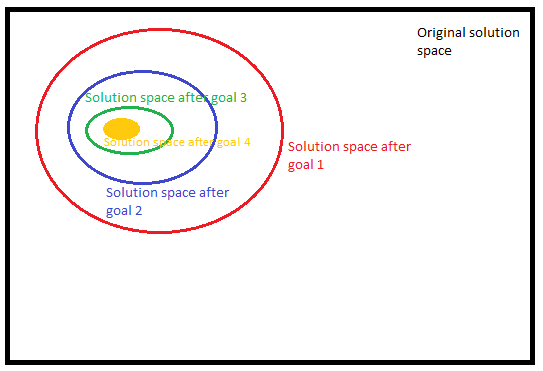
\includegraphics[scale=0.6]{figures/goalProgSpace.png}
\centering
\caption{Solution spaces are limited and encapsulated after each goal optimization step.}
\end{figure}

\fixme{atualizar etapas na figura}


%%%%%%%%%%%%%%
\subsubsection{Nonpreemptive Goal Programming}
\fixme{or Multi-objective function? no final nao tem mta diferenca!}

Following there is the unified objective function considered at this work. Although here it is even easier than at goal programming to change priorities order and adding or removing goals, there is the necessity of choosing coefficients for variables at objective function.

$$
\begin{array}{rl}
   \mbox{MIN} &
			\lambda \cdot \sum\limits_{a \in A}\sum\limits_{d \in D} \cdot fd_{d,a}
      \\
      &
      + \omega \cdot \sum\limits_{d \in D} 
\sum\limits_{t \in T} \sum\limits_{i \in I_{d}} (fkp_{d,i,k} + fkm_{d,i,k})
      \\
      &
      + \epsilon \cdot \sum\limits_{p \in P} \sum\limits_{t \in T} \sum\limits_{f \in F} fpgap_{p,t,f}
      \\
      &
			+ \sigma \cdot \sum\limits_{p \in P} \sum\limits_{t \in T} \sum\limits_{u1 \in U} \sum\limits_{u2 \in U} Time_{u1,u2} \cdot desloc_{p,t,u1,u2}
			\\
			&
      + \theta \cdot \sum\limits_{i \in I_{d}} \sum\limits_{d \in D} \sum\limits_{cp \in CP} y_{pv,i,d,cp}
\end{array}
$$


An unified objective function is more appropriate when goals have not a strict priority order, in the sense that their combinations can produce solutions that are Pareto efficient.

So, the question when choosing the approach is whether one wants to order or weight goals.


%%%%%%%%%%%%%%%%%%%%%%%%%%%%%%%%%%%%%
\subsection{Comparing results}

Through preemptive goal programming it is easier to understand the best solution found by the optimization process and the reasons of non-satisfaction of different goals, specially when the number of goals to be achieved through the objective function increases.





%%%%%%%%%%%%%%%%%%%%%%%%%%%%%%%%%%%%%%%%%%%%%%%%%%%%%%%%%%%%%%%%%%%%%%%%%%%%%%%%%%%%%%%%%%%%%%%%%%%
%%%%%%%%%%%%%%%%%%%%%%%%%%%%%%%%%%%%%%%%%%%%%%%%%%%%%%%%%%%%%%%%%%%%%%%%%%%%%%%%%%%%%%%%%%%%%%%%%%%
\section{Polishing Method}

%%%%%%%%%%%%%%%%%%%%%%%%%%%%%%%
\subsection{Definition}

Introduces polishing concept.

%%%%%%%%%%%%%%%%%%%%%%%%%%%%%%%%%%%%%
\subsection{Polishing method developed for the problem}

%%%%%%%%%%%%%%%%%%%%%%%%%%%%%%%%%%%%%
\subsection{Comparing different approaches}

%%%%%%%%%%%%%%%%%%%%%%%%%%%%%%%%%%%%%
\subsubsection{Fixing types}




%%%%%%%%%%%%%%%%%%%%%%%%%%%%%%%%%%%%%%%%%%%%%%%%%%%%%%%%%%%%%%%%%%%%%%%%%%%%%%%%%%%%%%%%%%%%%%%%%%%
%%%%%%%%%%%%%%%%%%%%%%%%%%%%%%%%%%%%%%%%%%%%%%%%%%%%%%%%%%%%%%%%%%%%%%%%%%%%%%%%%%%%%%%%%%%%%%%%%%%
\section{Root relaxation}

%%%%%%%%%%%%%%%%%%%%%%%%%%%%%%%%%%%%%
\subsection{Barrier method vs primal method algorithms}




%%%%%%%%%%%%%%%%%%%%%%%%%%%%%%%%%%%%%%%%%%%%%%%%%%%%%%%%%%%%%%%%%%%%%%%%%%%%%%%%%%%%%%%%%%%%%%%%%%%
%%%%%%%%%%%%%%%%%%%%%%%%%%%%%%%%%%%%%%%%%%%%%%%%%%%%%%%%%%%%%%%%%%%%%%%%%%%%%%%%%%%%%%%%%%%%%%%%%%%
\section{Different mathematical formulation}

%%%%%%%%%%%%%%%%%%%%%%%%%%%%%%%%%%%%%
\subsection{Single time slot variable vs grouping time slot variable}



As in all combinatorial scheduling models, the problem grows more complex as the number of side constraints increases.\fixme{Colocar essa frase no lugar adequado!}



%%%%%%%%%%%%%%%%%%%%%%%%%%%%%%%%%%%%%%%%%%%%%%%%%%%%%%%%%%%%%%%%%%%%%%%%%%%%%%%%%%%%%%%%%%%%%%%%%%%
%%%%%%%%%%%%%%%%%%%%%%%%%%%%%%%%%%%%%%%%%%%%%%%%%%%%%%%%%%%%%%%%%%%%%%%%%%%%%%%%%%%%%%%%%%%%%%%%%%%
\section{Usage of virtual resource}

%%%%%%%%%%%%%%%%%%%%%%%%%%%%%%%%%%%%%
\subsection{Virtual professor vs no virtual professors}


\chapter{Analysis of constraints' impacts}
\label{chap:constranalysis}


%%%%%%%%%%%%%%%%%%%%%%%%%%%%%%%%%%%%%%%%%%%%%%%%%%%%%%%%%%%%%%%%%%%%%%%%%%%%%%%%%
\section{Avoiding gaps in student's timetable}



%%%%%%%%%%%%%%%%%%%%%%%%%%%%%%%%%%%%%%%%%%%%%%%%%%%%%%%%%%%%%%%%%%%%%%%%%%%%%%%%%%
\section{Avoiding gaps in professor's timetable}



%%%%%%%%%%%%%%%%%%%%%%%%%%%%%%%%%%%%%%%%%%%%%%%%%%%%%%%%%%%%%%%%%%%%%%%%%%%%%%%%%%
\section{Allowing non-continuous course lessons at day}



%%%%%%%%%%%%%%%%%%%%%%%%%%%%%%%%%%%%%%%%%%%%%%%%%%%%%%%%%%%%%%%%%%%%%%%%%%%%%%%%%%
\section{Credits split rule}



%%%%%%%%%%%%%%%%%%%%%%%%%%%%%%%%%%%%%%%%%%%%%%%%%%%%%%%%%%%%%%%%%%%%%%%%%%%%%%%%%%
\section{Hard vs soft constraints}

\chapter{Converting and Comparing Formats}
\label{chap:converting}


%%%%%%%%%%%%%%%%%%%%%%%%%%%%%%%%%%%%%%%%%%%%%%%%%%%%%%%%%%%%%%%%%%%%%%%%%%%%%%%%%%

\section{XHSTT format}


%%%%%%%%%%%%%%%%%%%%%%%%%%%%%%%%%%%%%%%%%%%%%%%%%%%%%%%%%%%%%%%%%%%%%%%%%%%%%%%%%%

\section{Converting XHSTT problem into Trieda's problem}

\subsection{What was considered}

\subsection{What was not considered}


%%%%%%%%%%%%%%%%%%%%%%%%%%%%%%%%%%%%%%%%%%%%%%%%%%%%%%%%%%%%%%%%%%%%%%%%%%%%%%%%%%

\section{Solving a XHSTT instance with Trieda's solver}

\subsection{Results}


%%%%%%%%%%%%%%%%%%%%%%%%%%%%%%%%%%%%%%%%%%%%%%%%%%%%%%%%%%%%%%%%%%%%%%%%%%%%%%%%%%


\chapter{Computational Experiments}
\label{chap:experiments}


This chapter describes the main computational experiments made in this work. First, general computational aspects are introduced; then different scenarios for different schools are described; and finally results are presented and evaluated.


%%%%%%%%%%%%%%%%%%%%%%%%%%%%%%%%%%%%%%%%%%%%%%%%%%%%%%%%%%%%%%%%%%%%%%%%%%%%%%%%%%
\section{General}

The implementation of the solver was done in C++, compiled with MS Visual Studio 2010 environment, using Microsoft Windows 7, 64 bits.

All the linear integer programs were solved using the generic MIP-Solver Gurobi 6.0. 

Computational experiments were executed on 3.40GHz Intel Core i7 computer with 32 GB of RAM. Considering all scenarios, the maximum observed amount of RAM being used by the solver during execution was around 7 GB.


%%%%%%%%%%%%%%%%%%%%%%%%%%%%%%%%%%%%%%%%%%%%%%%%%%%%%%%%%%%%%%%%%%%%%%%%%%%%%%%%%%
\section{Scenarios}

Several computational experiments have been performed for real scenarios of Brazilian schools. Those considered the most significant are following detailed.

General features of scenarios:
\begin{table}[ht]
\caption{Scenarios} 							% title of Table
\centering
\begin{tabular}{c c c c c} 							% centered columns
\hline\hline 											% inserts double horizontal lines
Scenario & Classes & Credits demanded & Teaching staff available credits & Blocks \\ [0.5ex] 						% heading
\hline 														% inserts single horizontal line
A & 178 & 5800 & 9154 & 14 \\
B1 & 295 & 9490 & 15249 & 15 \\
B2 & 295 & 9490 & 15243 & 15 \\
C & & & & \\
D & & & & \\
E & & & & \\ [1ex] 							% [1ex] adds vertical space
\hline
\end{tabular}
\label{table:scenarios} 					% is used to refer this table in the text
\end{table}



Detailed features of scenarios:
\begin{table}[ht]
\caption{Scenarios} 							% title of Table
\centering
\begin{tabular}{c | c c c c c c} 	% centered columns
\hline\hline 											% inserts double horizontal lines
\multirow{2}{*}{Features} &
	\multicolumn{6}{c}{Scenarios} \\
																				& A & B1 & B2 & C & D & E \\ [0.5ex] 						% heading
\hline 														% inserts single horizontal line
Classes 																& 178	& 295	 & 295& & \\
Demanded credits 												& 5800	& 9490 & 9490& & \\
Average of demanded credits per class 	& 32.5843	& 32.1695	 & 32.1695& & \\
\hline
Professors 															& 	& 	 & & & \\
Professors available credits 						& 9154	& 15249	 & 15243& & \\
1st-priority professors available credits & 	& 	 & & & \\
2nd-priority professors available credits	& 	& 	 & & & \\
\hline
Blocks 																	& 14	& 15	 & 15& & \\
Min/Max classes per block 							& 2/29	& 9/28 & 9/28& & \\
Average of classes per block 						& 	& 	 & & & \\

 [1ex] 							% [1ex] adds vertical space
\hline
\end{tabular}
\label{table:scenarios} 					% is used to refer this table in the text
\end{table}




\begin{enumerate}
%---------------
\item A: Pensi - sem noite - com amarracao de disponib por unidade

\begin{figure}[H]
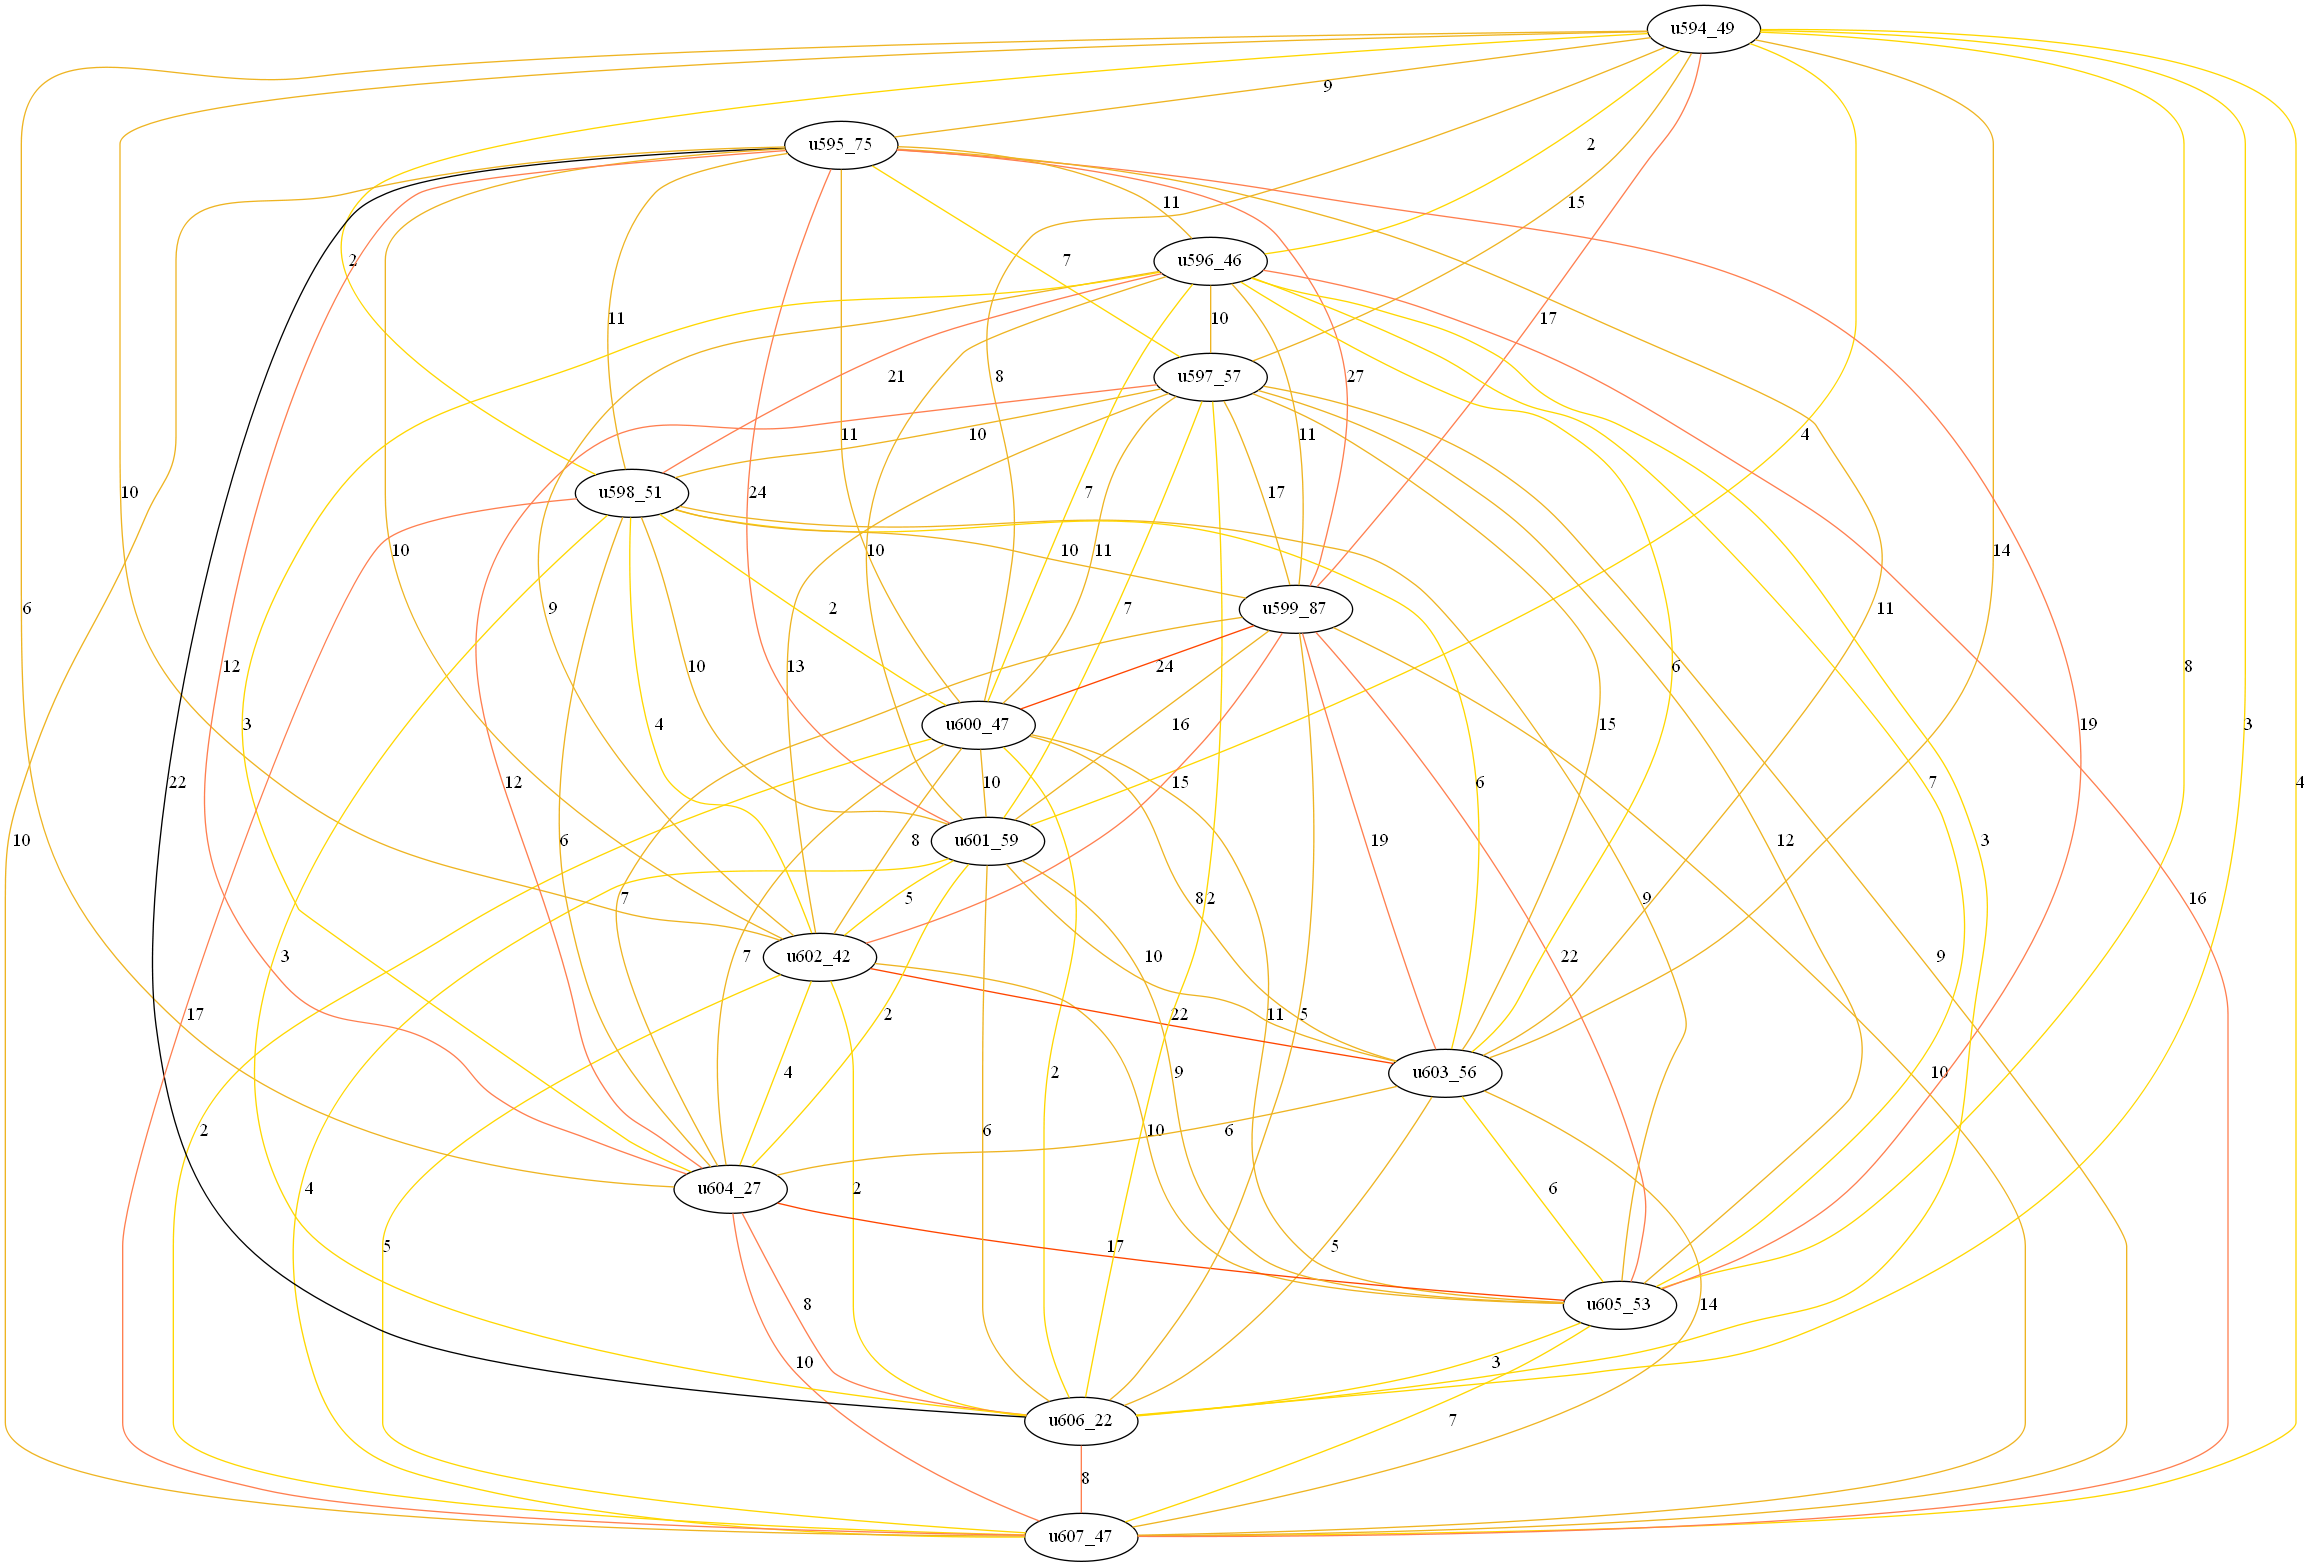
\includegraphics[scale=1.0]{"Computational Experiments/Inputs/inputPensiSemNoitePriorProfs_201501291331550_/parUnidProfsComuns-PensiSemNoitePriorProfs_201501291331550.png"}
\centering
\caption{Sharing of professors between blocks (school units) of scenario A}
\end{figure}

%---------------
\item B1: Elite - sem amarracao de disponib por unidade

\begin{figure}[H]
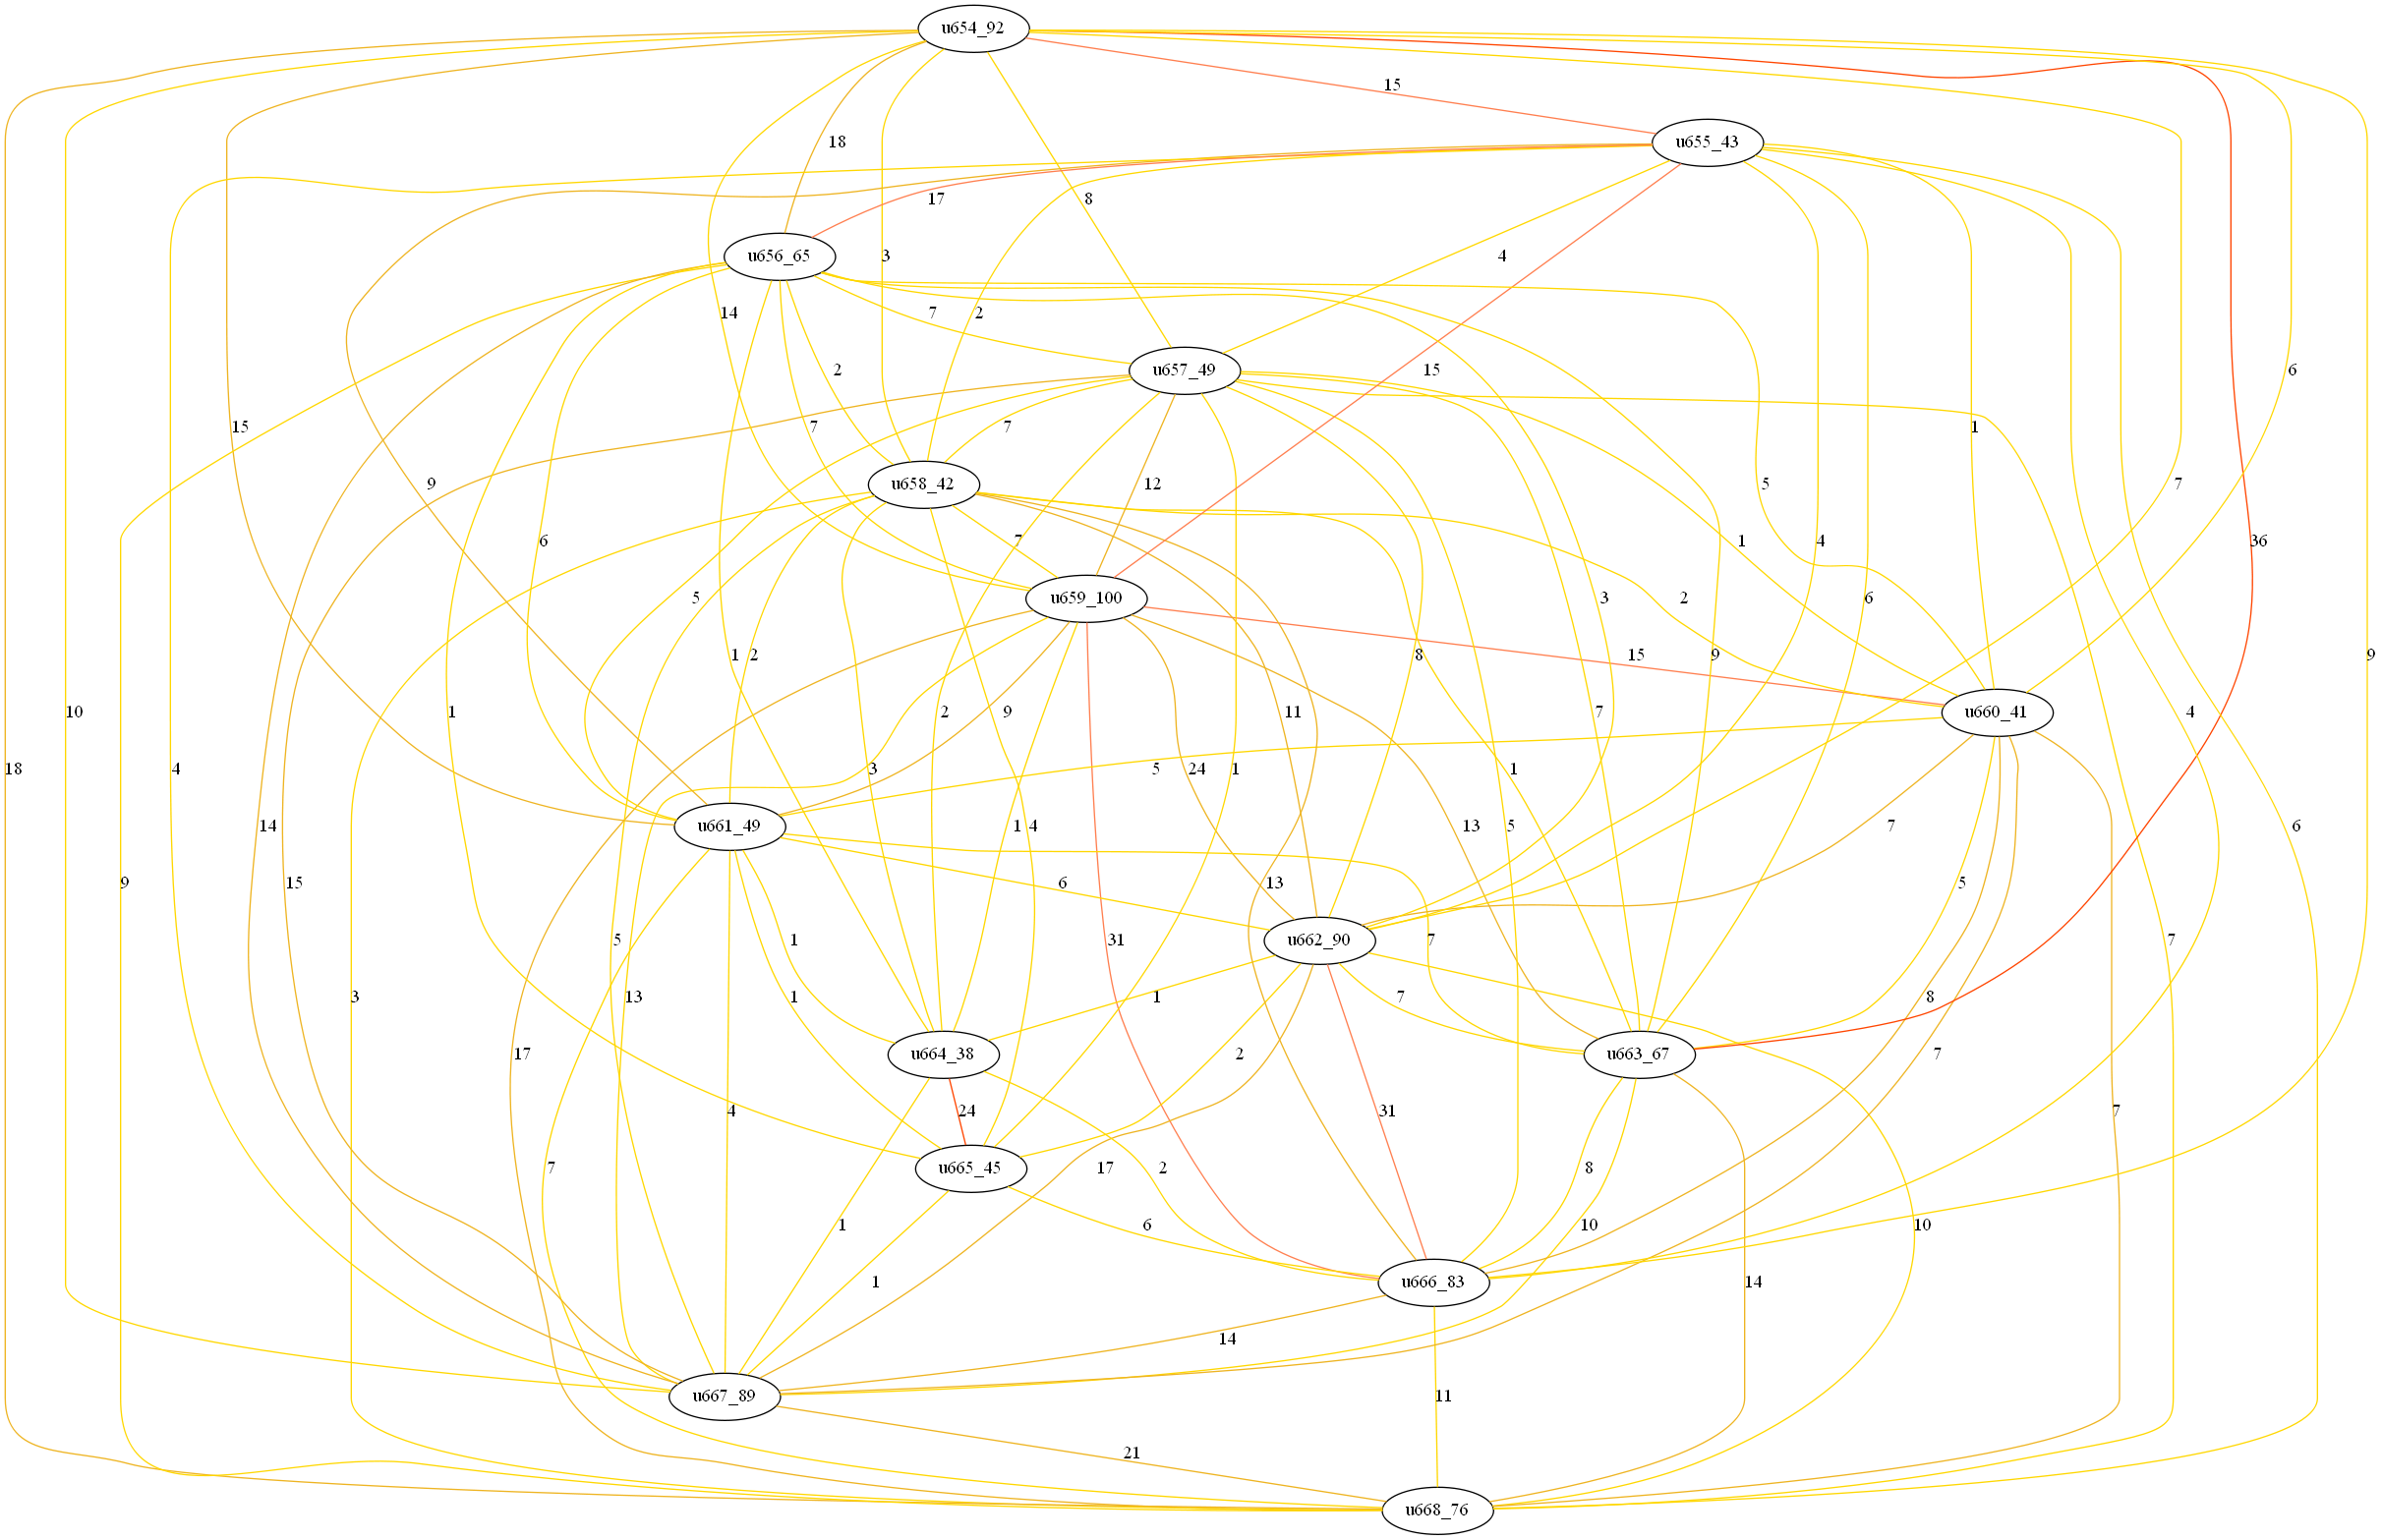
\includegraphics[scale=1.0]{"Computational Experiments/Inputs/inputEliteComPriorProfSemDispUn_201502011233270_/parUnidProfsComuns-EliteComPriorProfSemDispUn_201502011233270.png"}
\centering
\caption{Sharing of professors between blocks (school units) of scenario B1}
\end{figure}


%---------------
\item B2: Elite - com amarracao de disponib por unidade

\begin{figure}[H]
\includegraphics[scale=1.0]{"Computational Experiments/Inputs/inputEliteComPriorProfs_201501300027330_/parUnidProfsComuns-EliteComPriorProfs_201501300027330.png"}
\centering
\caption{Sharing of professors between blocks (school units) of scenario B2}
\end{figure}


%---------------
\item C: Elite ou Pensi - exemplo pequeno

%---------------
\item D: CEI

%---------------
\item E: Colegio Vicosa

\end{enumerate}


%%%%%%%%%%%%%%%%%%%%%%%%%%%%%%%%%%%%%%%%%%%%%%%%%%%%%%%%%%%%%%%%%%%%%%%%%%%%%%%%%%
\section{Approaches}

Different approaches and strategies for solving the problem were discussed at chapter ~\ref{chap:strategies}. Here some of these approaches are combined so that further various computational experiments are carried out and impacts of these distinct strategies are evaluated. The variations to be combined are briefly reviewed below.

\paragraph{Preemptive and Nonpreemptive Goal Programming}
The impact of ordered goals, their correlations, and trade-off situations are evaluated by solving the problem both with the preemptive goal programming and with an unified objective function.

\paragraph{Polishing method usage}
The need of the polishing method is demonstrated by optimizing the problem with and without it.

\paragraph{Professor Priority}
Professors priorities are evaluated using the three following perspectives:
\begin{enumerate}
\item No professor priority is considered: every goal of the problem is executed only once, considering all professors assignments without distinction.
\item Weak professor priority is considered: every goal of the problem is executed only once, but considering first-priority professors assignments more important than second-priority professors.
\item Strong professor priority is considered: every goal of the problem is executed twice. First, all goals are sequentially performed for all first-priority professors, then solution quality that was achieved for these professors is ensured and all goals are again sequentially performed for all second-priority professors.
\end{enumerate}

%Testes:
%
%23-02-15-NaraMaster-PensiSemNoitePriorProfs_201501291331550-priorTypeOff (Judas)
%21-02-15-NaraMaster-PensiSemNoitePriorProfs_201501291331550-priorTypeOffWeight (Slayer)
%21-02-15-NaraMaster-PensiSemNoitePriorProfs_201501291331550-priorType2 (Judas)
%
%23-02-15-NaraMaster-EliteComPriorProfSemDispUn_201502011233270-priorTypeOff (Slayer)
%22-02-15-NaraMaster-EliteComPriorProfSemDispUn_201502011233270-priorType2 (Slayer)
%24-02-15-NaraMaster-EliteComPriorProfSemDispUn_201502011233270-priorTypeOffWeight (PadreMarcelo)
%
%24-02-15-NaraMaster-EliteComPriorProfs_201501300027330-priorTypeOff (Slayer)
%26-02-14-NaraMaster-EliteComPriorProfs_201501300027330-priorType2 (PadreMarcelo rodando)
%26-02-14-NaraMaster-EliteComPriorProfs_201501300027330-priorTypeOffWeight (Slayer rodando)
%
%23-02-14-NaraMaster-PensiSemNoiteProfsImpo_201501291331550-priorTypeOffWeight (PadreMarcelo)

%%%%%%%%%%%%%%%%%%%%%%%%%%%%%%%%%%%%%%%%%%%%%%%%%%%%%%%%%%%%%%%%%%%%%%%%%%%%%%%%%%
\section{Results}

\subsection{Model features}

Following, model features for each instance are listed, which include the number of variables and restrictions created, detailed by type, and the reduced size of the model after applying Gurobi pre-solve method.


\subsection{Solver performance}

Whenever the solver is executed, analyzing performance and consequently the generated solution implies in analyzing every solving phase. This means checking for every step the running time, the optimization stopping condition that was reached, the best solution value of the linear program, the optimality gap and also how the solving process converged during the polishing method.


\subsection{Solution quality}

Evaluating quality of a final solution is not a trivial task, specially because there are multiple and conflicting goals involved. Often analyzing and understanding solutions require a deeper analysis of the problem data itself.

Following several solution quality indicators are listed and detailed for the experiments made.




\bibliography{dissertation}
\end{document}

